\chapter{Développement}

Cette section présente l'implémentation technique de SecuCom, en détaillant l'architecture de l'application, les modèles de données, les contrôleurs et services, ainsi que les fonctionnalités principales et les mécanismes de sécurité.

\section{Architecture de l'application}

\subsection{Vue d'ensemble}

L'implémentation de SecuCom suit une architecture en couches clairement séparées, permettant une meilleure organisation du code, une maintenance facilitée et une évolution plus souple du système. Cette architecture s'articule autour de cinq couches principales :

\vspace{0.5cm}

\begin{itemize}[leftmargin=*,label=\textcolor{darkgray}{$\bullet$},itemsep=0.3em]
  \item \textbf{Couche Modèle} : Représente les entités métier et leurs relations, implémentée via des classes Java annotées avec JPA.
  \item \textbf{Couche Repository} : Fournit les mécanismes d'accès aux données via Spring Data JPA, permettant d'abstraire les opérations de persistance.
  \item \textbf{Couche Service} : Contient la logique métier de l'application, orchestrant les opérations entre les repositories et les contrôleurs.
  \item \textbf{Couche DTO} : Assure la transformation des données entre la couche service et la couche contrôleur, permettant de découpler les modèles internes des représentations externes.
  \item \textbf{Couche Contrôleur} : Expose les API REST qui permettent aux clients (frontend) d'interagir avec le système.
\end{itemize}

\vspace{0.5cm}

\begin{tcolorbox}[
  title={\textbf{Architecture sécurisée}},
  colback=blue!5!white,
  colframe=primarycolor,
  fonttitle=\bfseries,
  boxrule=0.5mm,
  arc=2mm,
  left=6mm,
  right=6mm,
  top=6mm,
  bottom=6mm
]
Cette architecture est complétée par une couche transversale de sécurité qui gère l'authentification et l'autorisation à travers toutes les couches de l'application, assurant une protection cohérente des données et des fonctionnalités.
\end{tcolorbox}

\newpage

\noindent Le flux de données typique dans l'application suit le parcours suivant :

\begin{enumerate}[itemsep=0.3em]
  \item Le client (frontend) envoie une requête HTTP à un endpoint REST.
  \item La requête traverse d'abord la couche de sécurité qui vérifie l'authentification et les autorisations.
  \item Le contrôleur approprié reçoit la requête, valide les données d'entrée et les transmet au service correspondant.
  \item Le service applique la logique métier nécessaire et interagit avec les repositories pour accéder aux données.
  \item Les repositories communiquent avec la base de données via JPA/Hibernate.
  \item Le résultat remonte la chaîne : repository → service → contrôleur, avec les transformations DTO appropriées.
  \item Le contrôleur renvoie une réponse HTTP formatée au client.
\end{enumerate}

\vspace{0.5cm}

\begin{note}
Cette séparation des responsabilités permet non seulement une meilleure organisation du code, mais facilite également les tests unitaires et d'intégration, chaque couche pouvant être testée indépendamment.
\end{note}

\subsubsection{Organisation du frontend}

\vspace{0.5cm}

\noindent Le frontend de SecuCom est divisé en deux espaces distincts correspondant aux deux principaux rôles d'utilisateurs :

\begin{itemize}[leftmargin=*,label=\textcolor{darkgray}{$\bullet$},itemsep=0.3em]
  \item \textbf{Espace Secrétariat Social} : Accessible aux utilisateurs ayant le rôle \texttt{ROLE\_SECRETARIAT}, cet espace permet la gestion de toutes les entreprises clientes, leurs collaborateurs et leurs déclarations DIMONA.
  \item \textbf{Espace Entreprise} : Accessible aux utilisateurs ayant le rôle \texttt{ROLE\_COMPANY}, cet espace est limité aux données de l'entreprise à laquelle l'utilisateur est associé.

\end{itemize}

\vspace{0.5cm}

Cette séparation est implémentée au niveau du routage dans l'application React, avec des routes protégées qui vérifient le rôle de l'utilisateur avant d'autoriser l'accès. Bien que les deux espaces soient distincts en termes de données accessibles, ils partagent la même interface utilisateur (UI) pour maintenir une expérience cohérente. Les composants React sont réutilisés entre les deux espaces, mais les données affichées sont filtrées en fonction du rôle de l'utilisateur.

\vspace{0.5cm}

\begin{note}
Par exemple, le même composant de liste de collaborateurs est utilisé dans les deux espaces, mais dans l'espace Secrétariat Social, il peut afficher les collaborateurs de toutes les entreprises (avec possibilité de filtrer par entreprise), tandis que dans l'espace Entreprise, il n'affiche que les collaborateurs de l'entreprise de l'utilisateur connecté.
\end{note}

\begin{figure}[H]
  \centering
  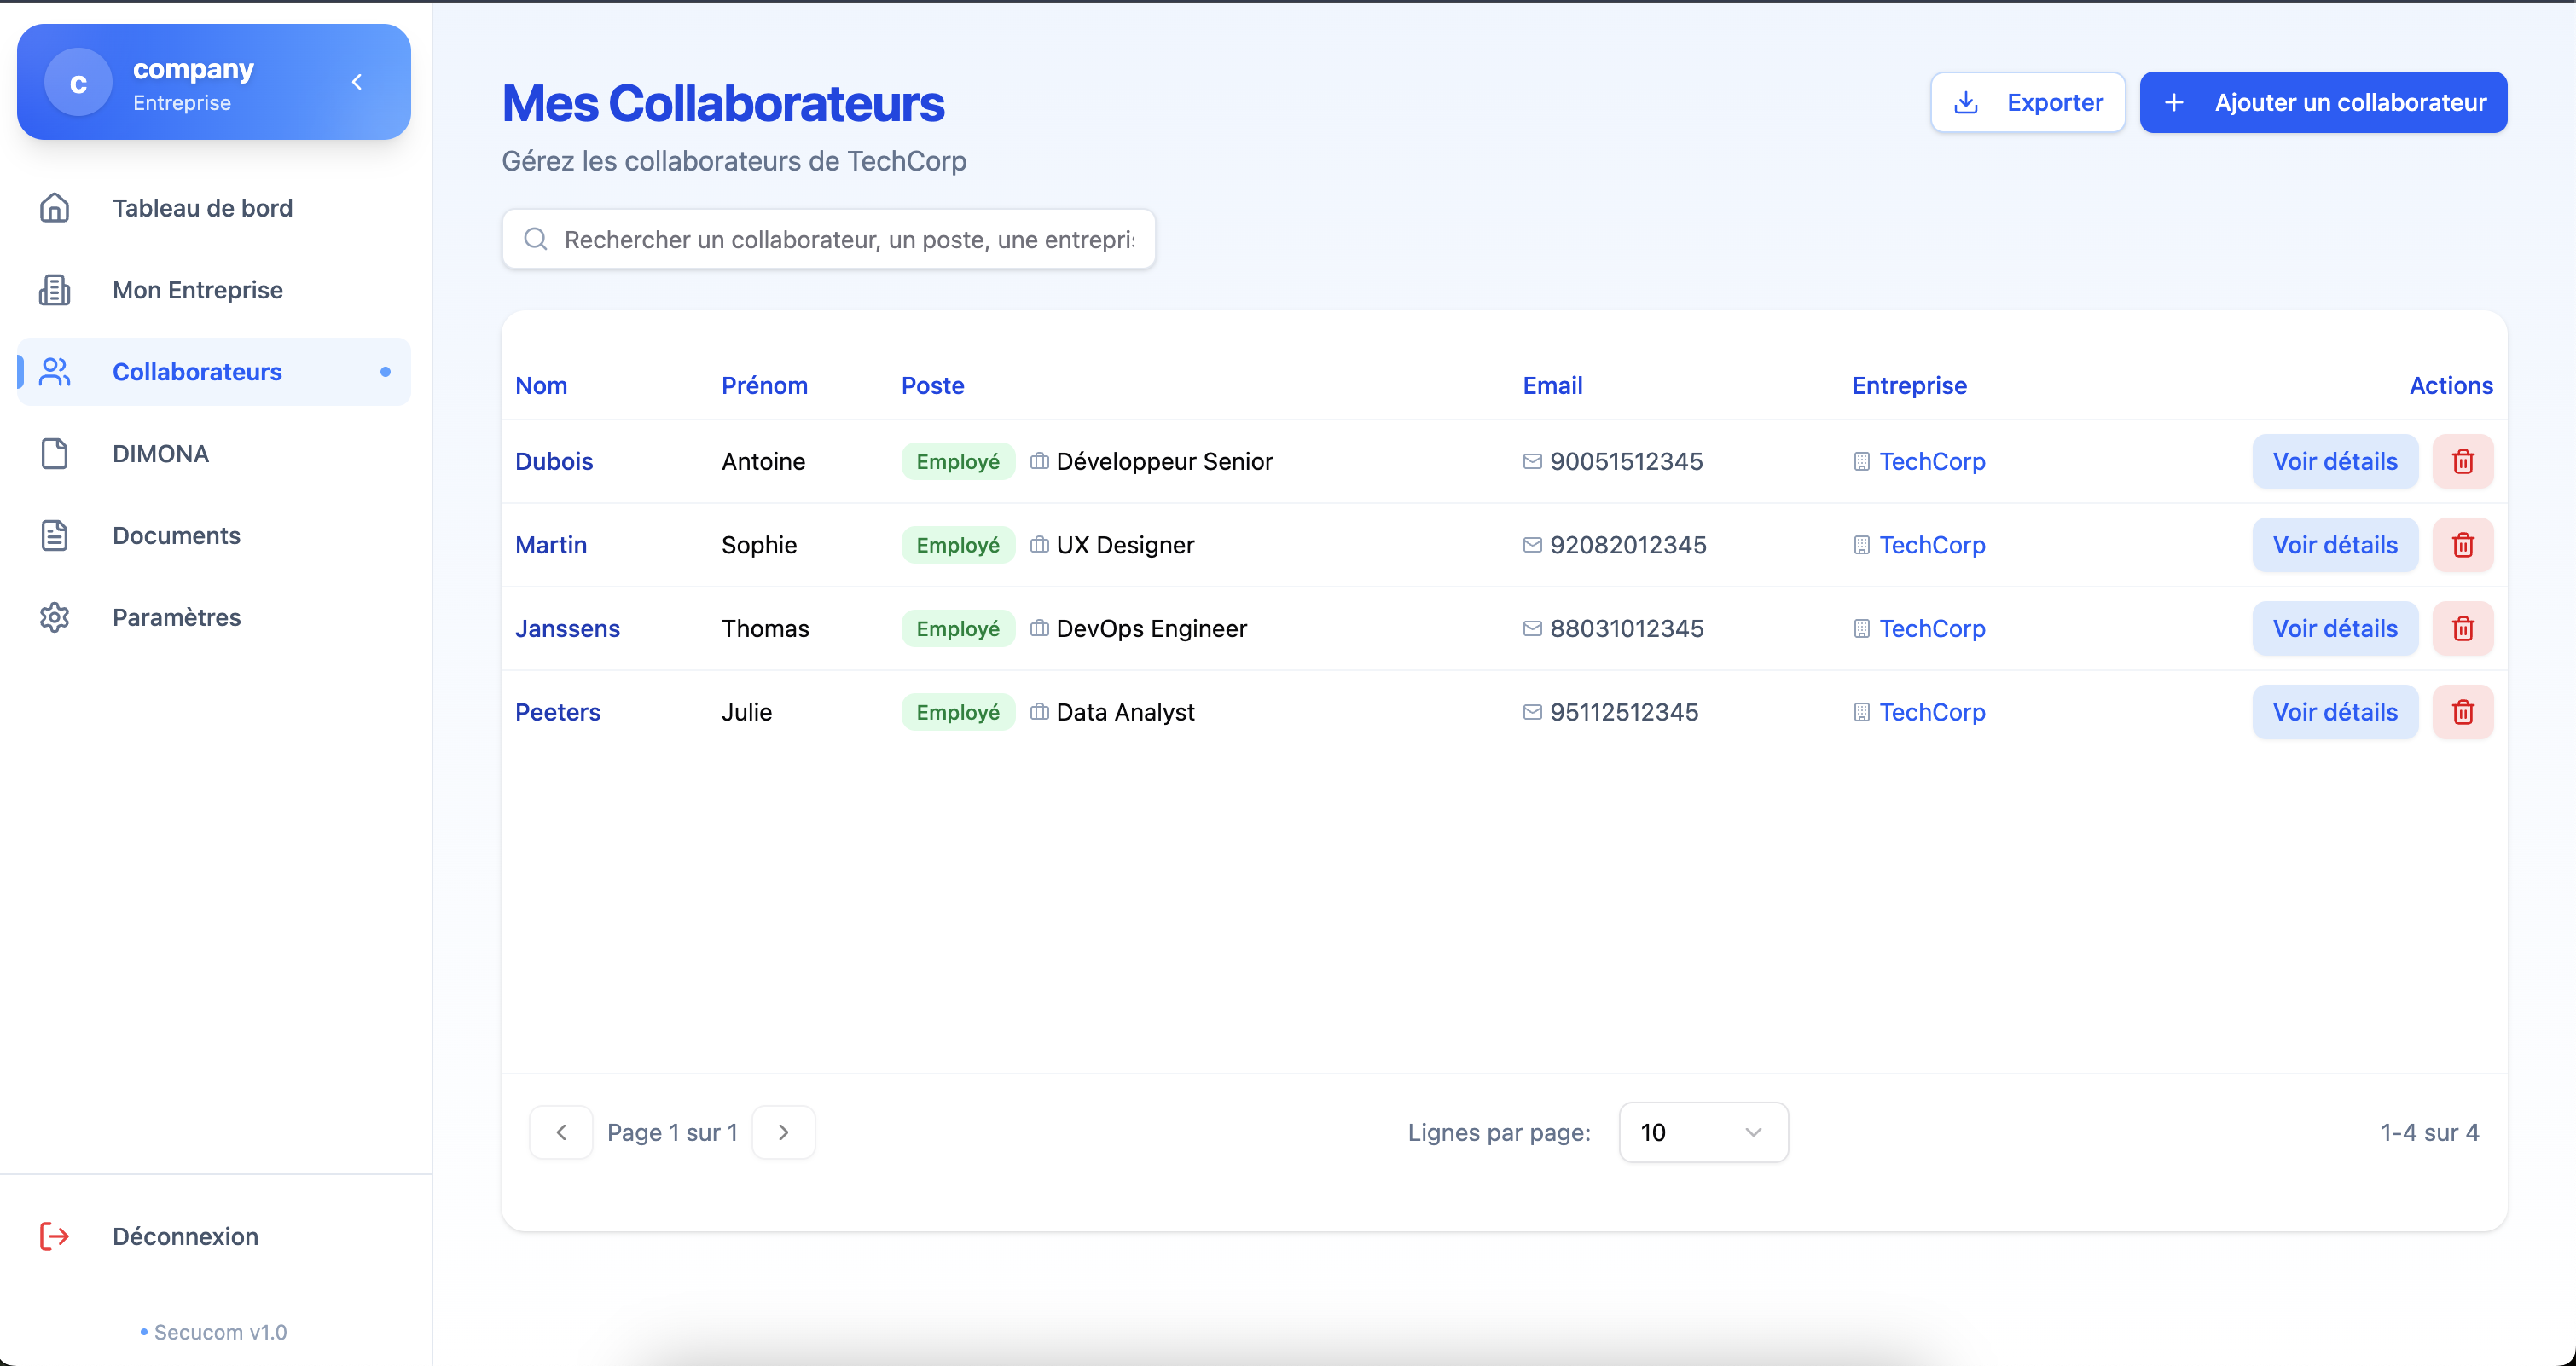
\includegraphics[width=1\textwidth]{SecuComPreviewCompanySpace.png}
  \caption{Aperçu de l'espace Entreprise}
  \label{fig:secucomPreviewUI}
\end{figure}

\vspace{0.5cm}

\begin{figure}[H]
  \centering
  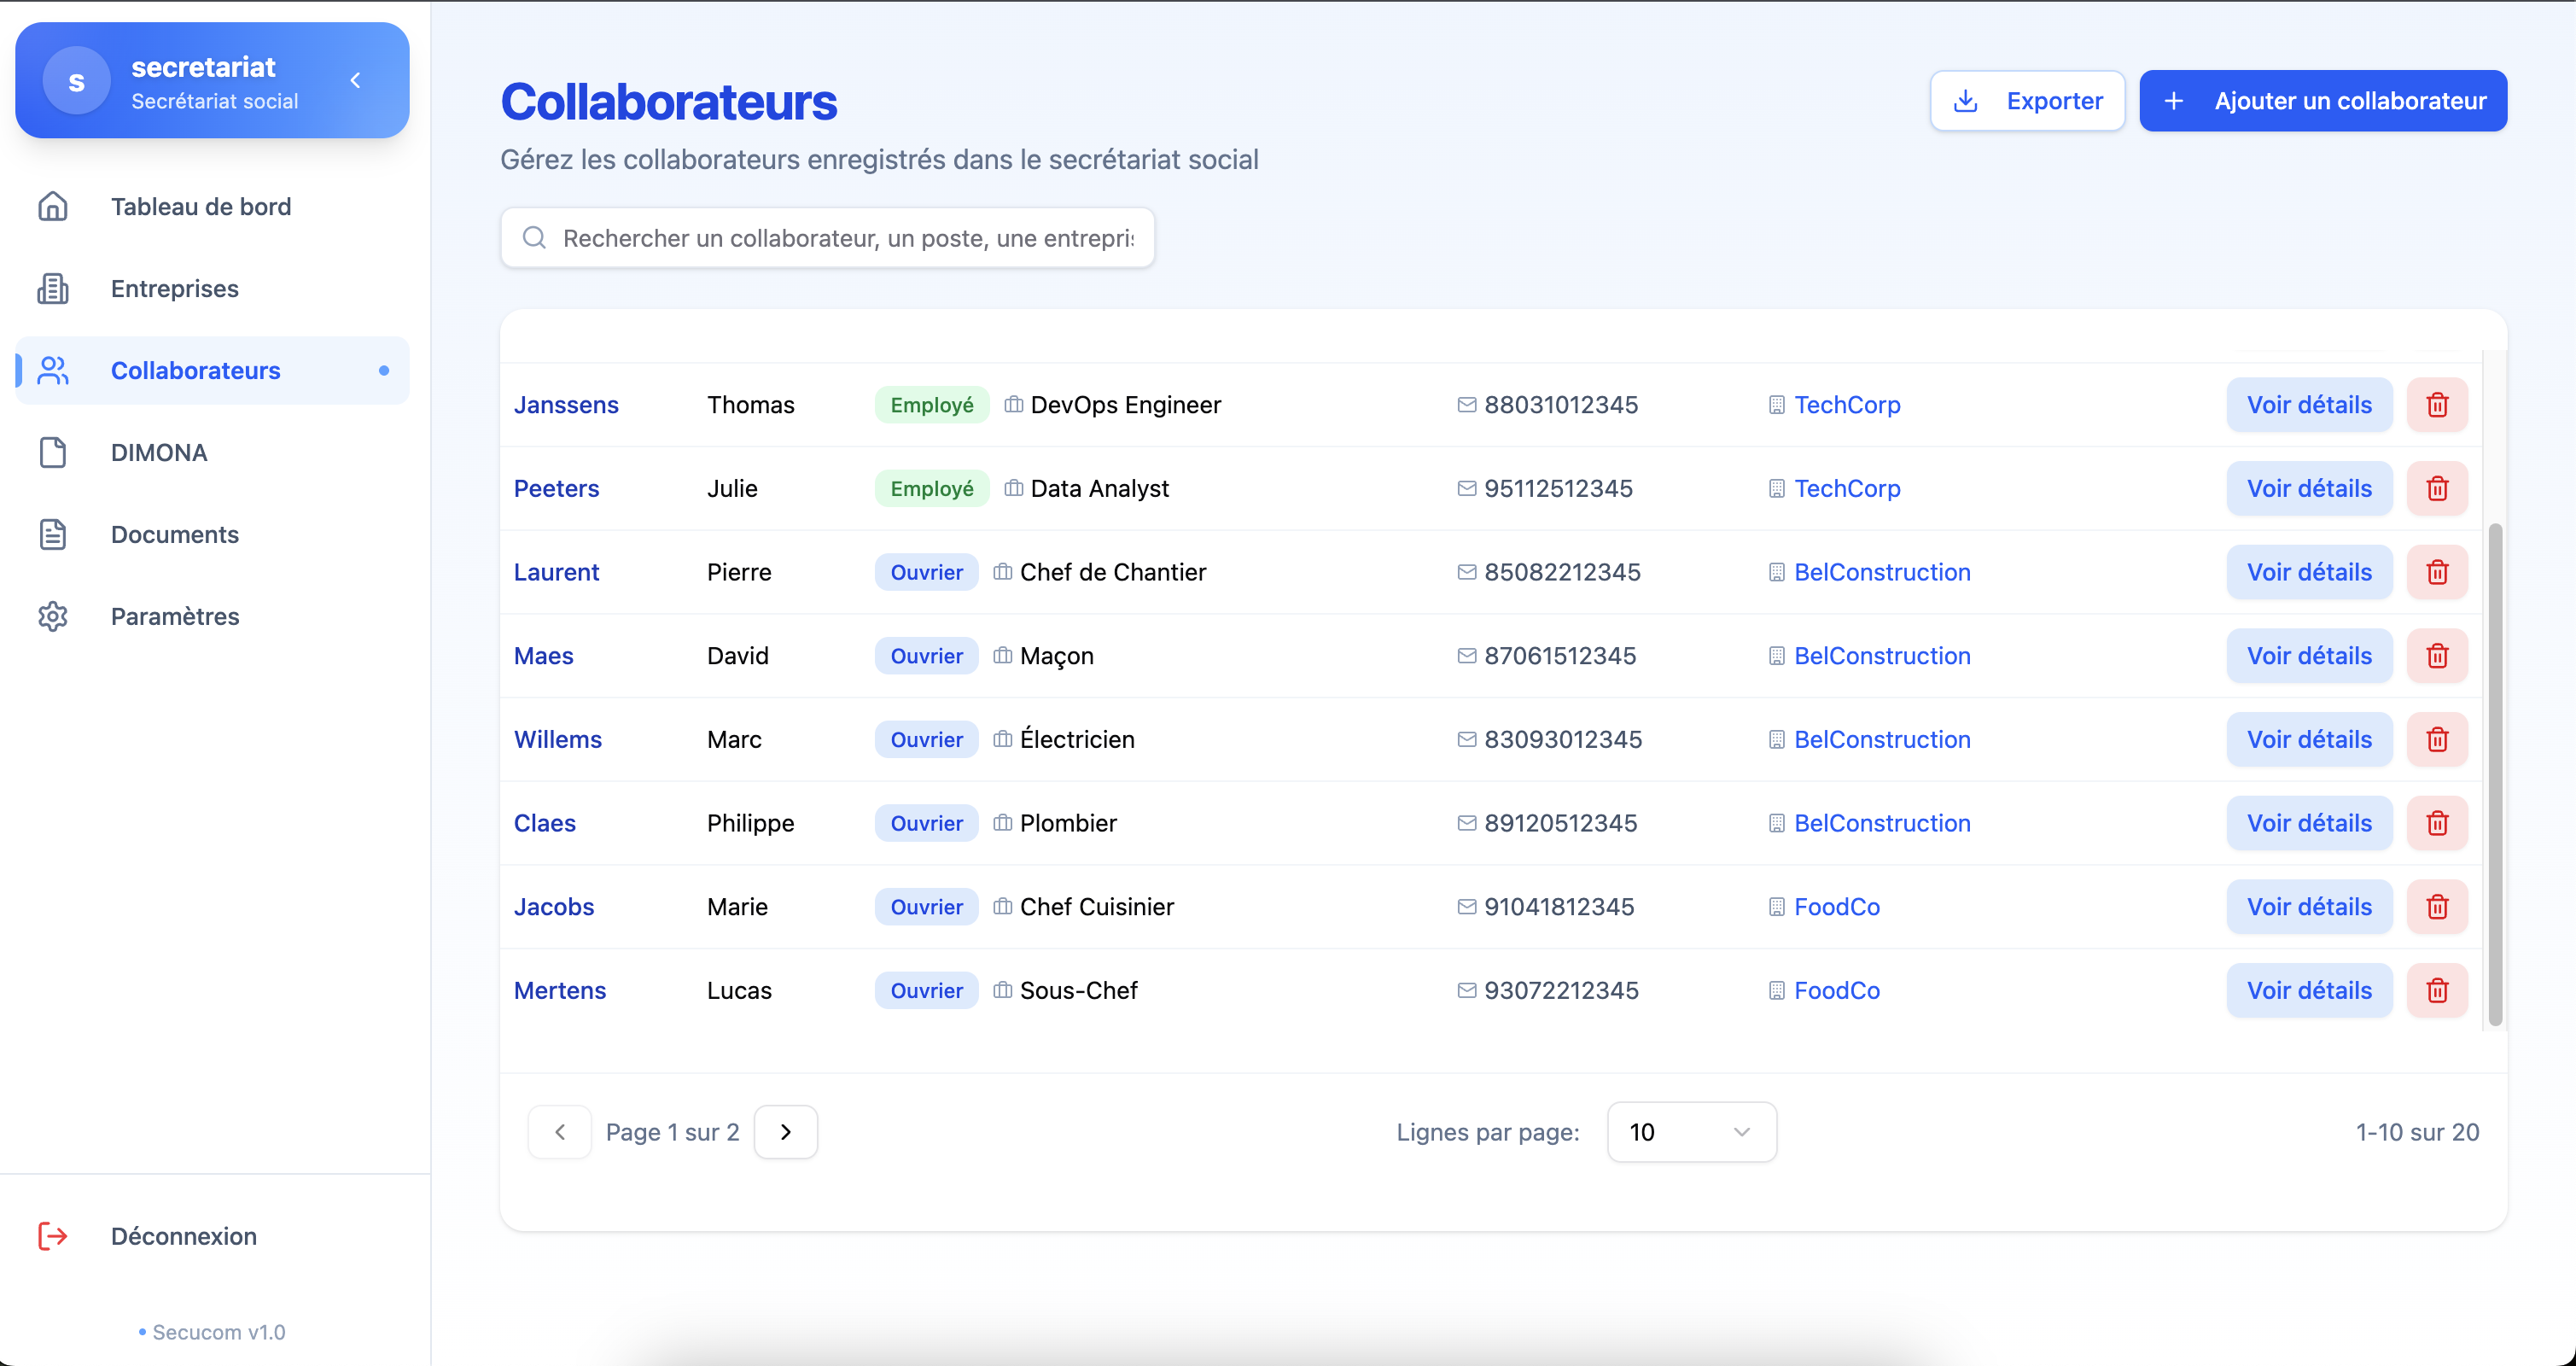
\includegraphics[width=1\textwidth]{SecuComPreviewSecretariatSpace.png}
  \caption{Aperçu de l'espace Secretariat social}
  \label{fig:secucomPreviewUI}
\end{figure}

\subsection{Modèles de données}

Les modèles de données constituent le cœur de l'application SecuCom. Ils représentent les entités métier et leurs relations, et sont implémentés sous forme de classes Java annotées avec JPA (Java Persistence API) pour la persistance en base de données.

\subsubsection{Entité User}

L'entité \texttt{User} représente la base de tous les utilisateurs du système. Elle utilise l'héritage avec une stratégie de table unique (\texttt{SINGLE\_TABLE}) pour différencier les types d'utilisateurs via une colonne discriminante.

\vspace{0.5cm}

\begin{figure}[H]
  \centering
  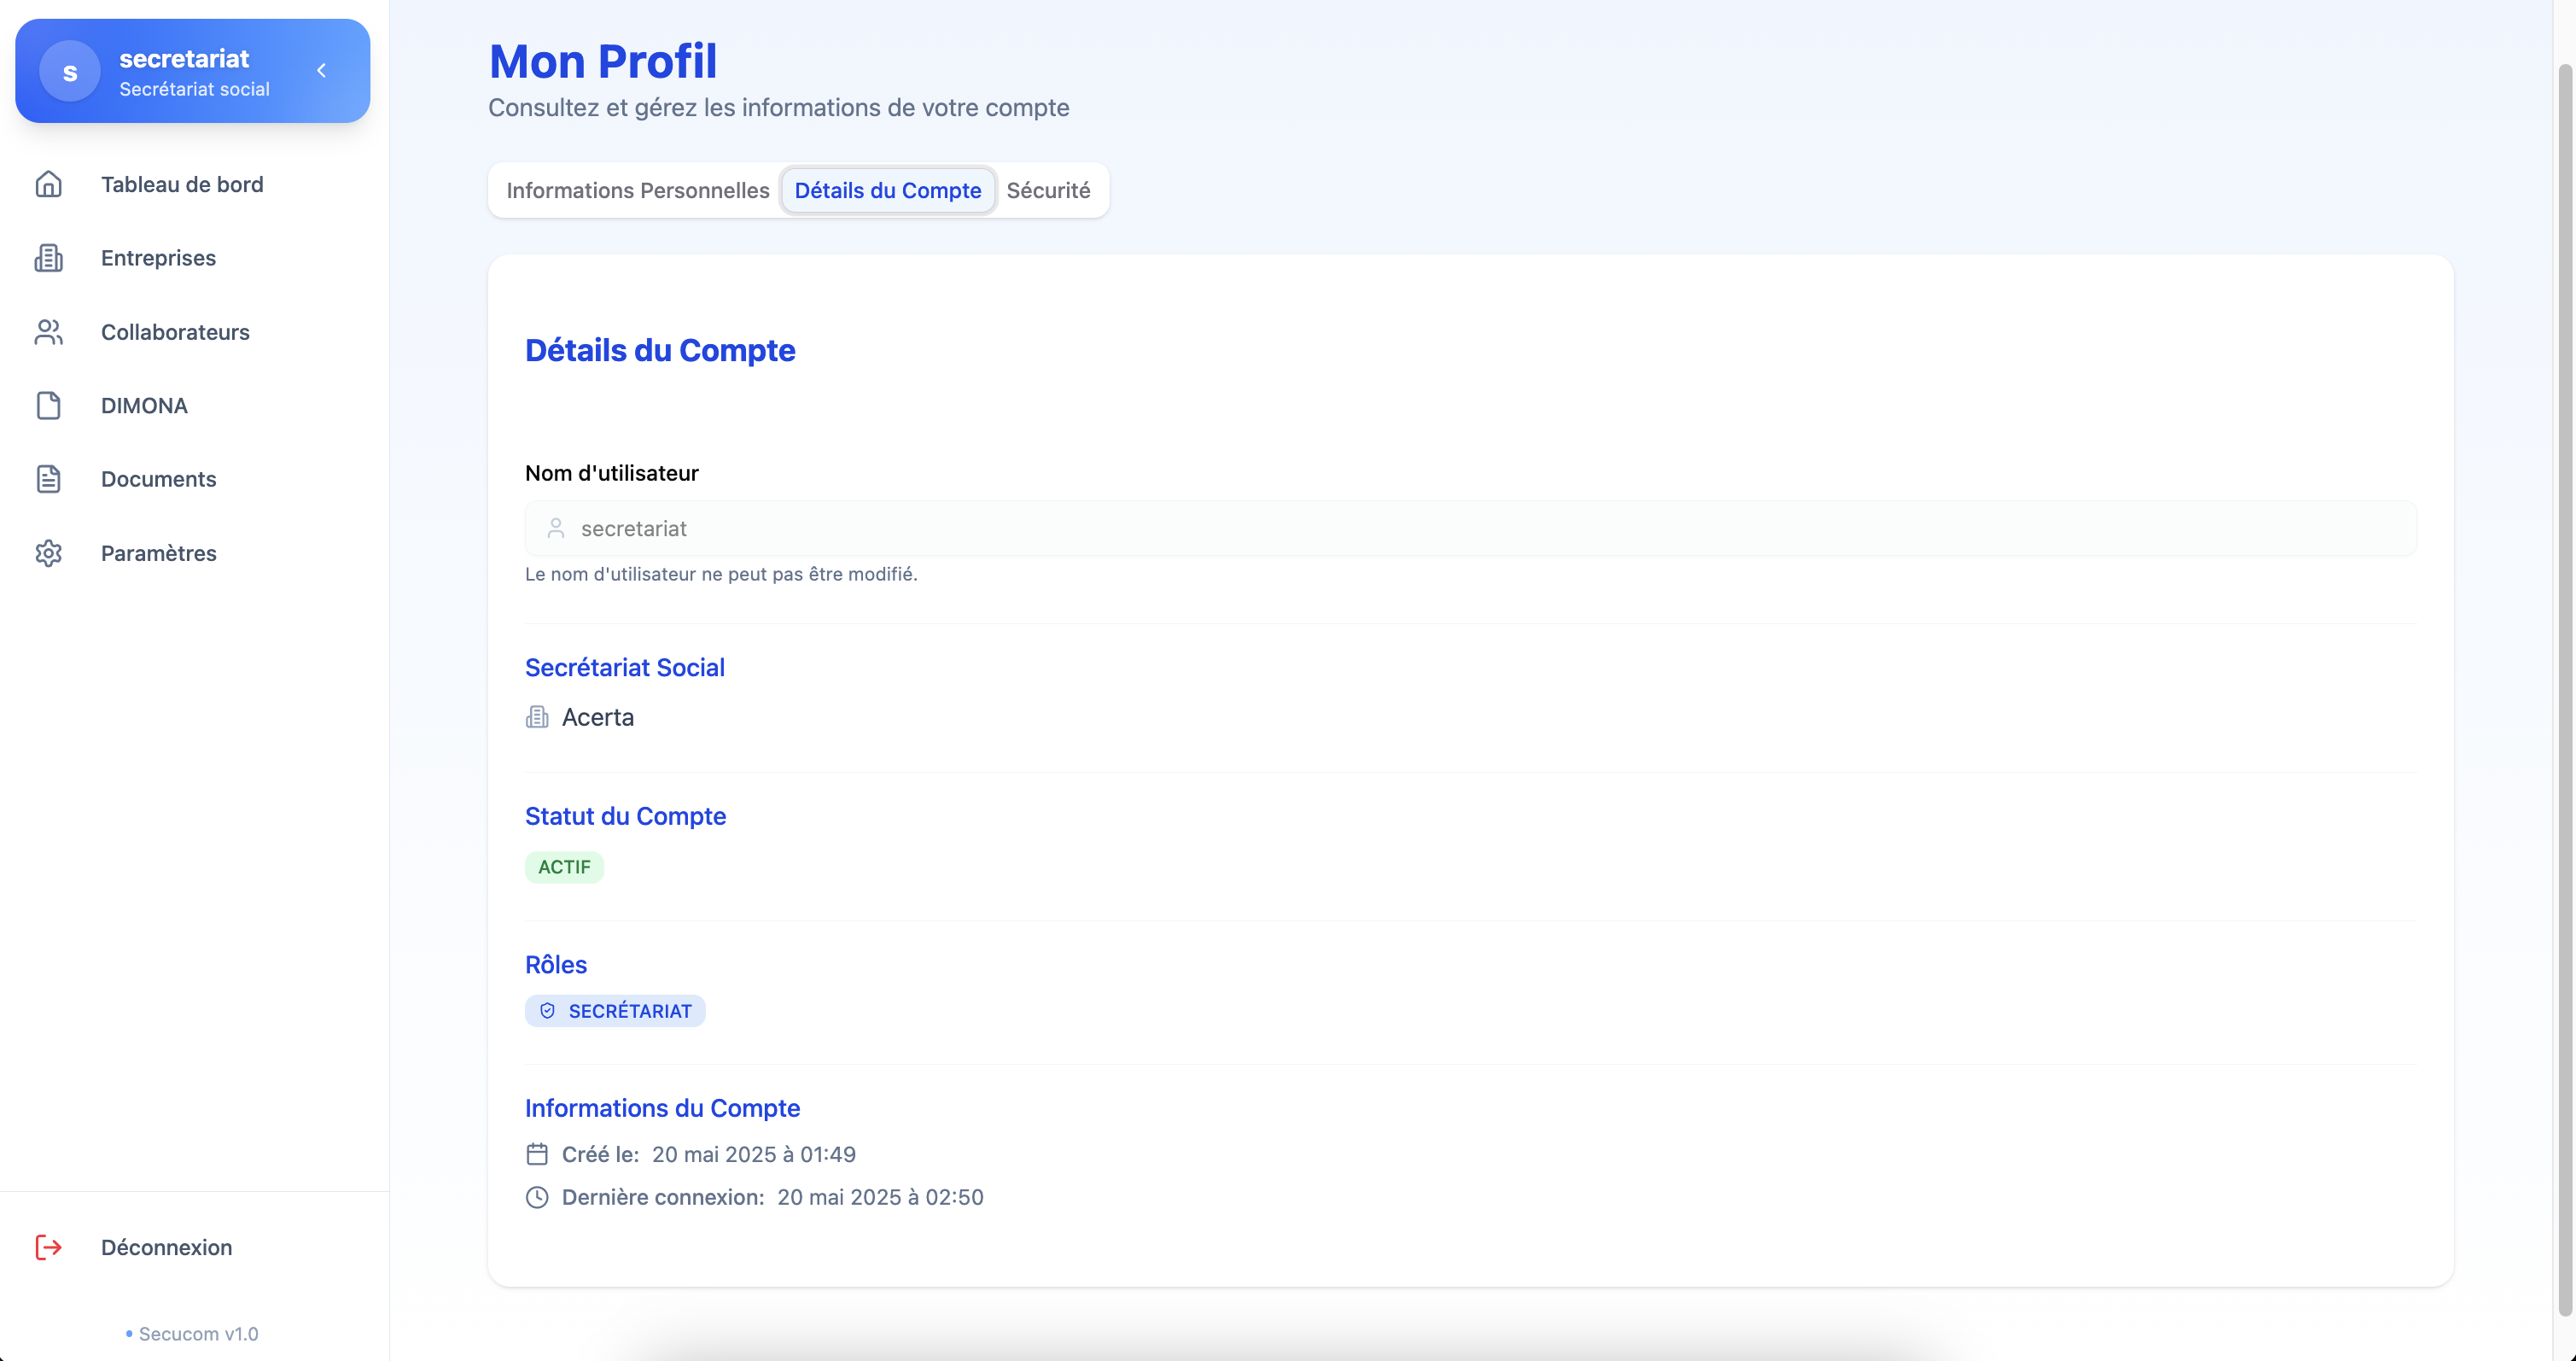
\includegraphics[width=1\textwidth]{SecuComPreviewUserProfile.png}
  \caption{Interface de gestion du profil utilisateur dans SecuCom}
  \label{fig:companyInterface}
\end{figure}

\vspace{0.5cm}

\begin{note}
Cette approche d'héritage permet de spécialiser les utilisateurs en différents types (employés du secrétariat, contacts d'entreprise) tout en maintenant une base commune pour l'authentification et les informations de base.
\end{note}

\subsubsection{Entité Company}

L'entité \texttt{Company} représente une entreprise cliente du secrétariat social. Elle contient de nombreux attributs reflétant les informations administratives et légales nécessaires.

\vspace{0.5cm}

\begin{figure}[H]
  \centering
  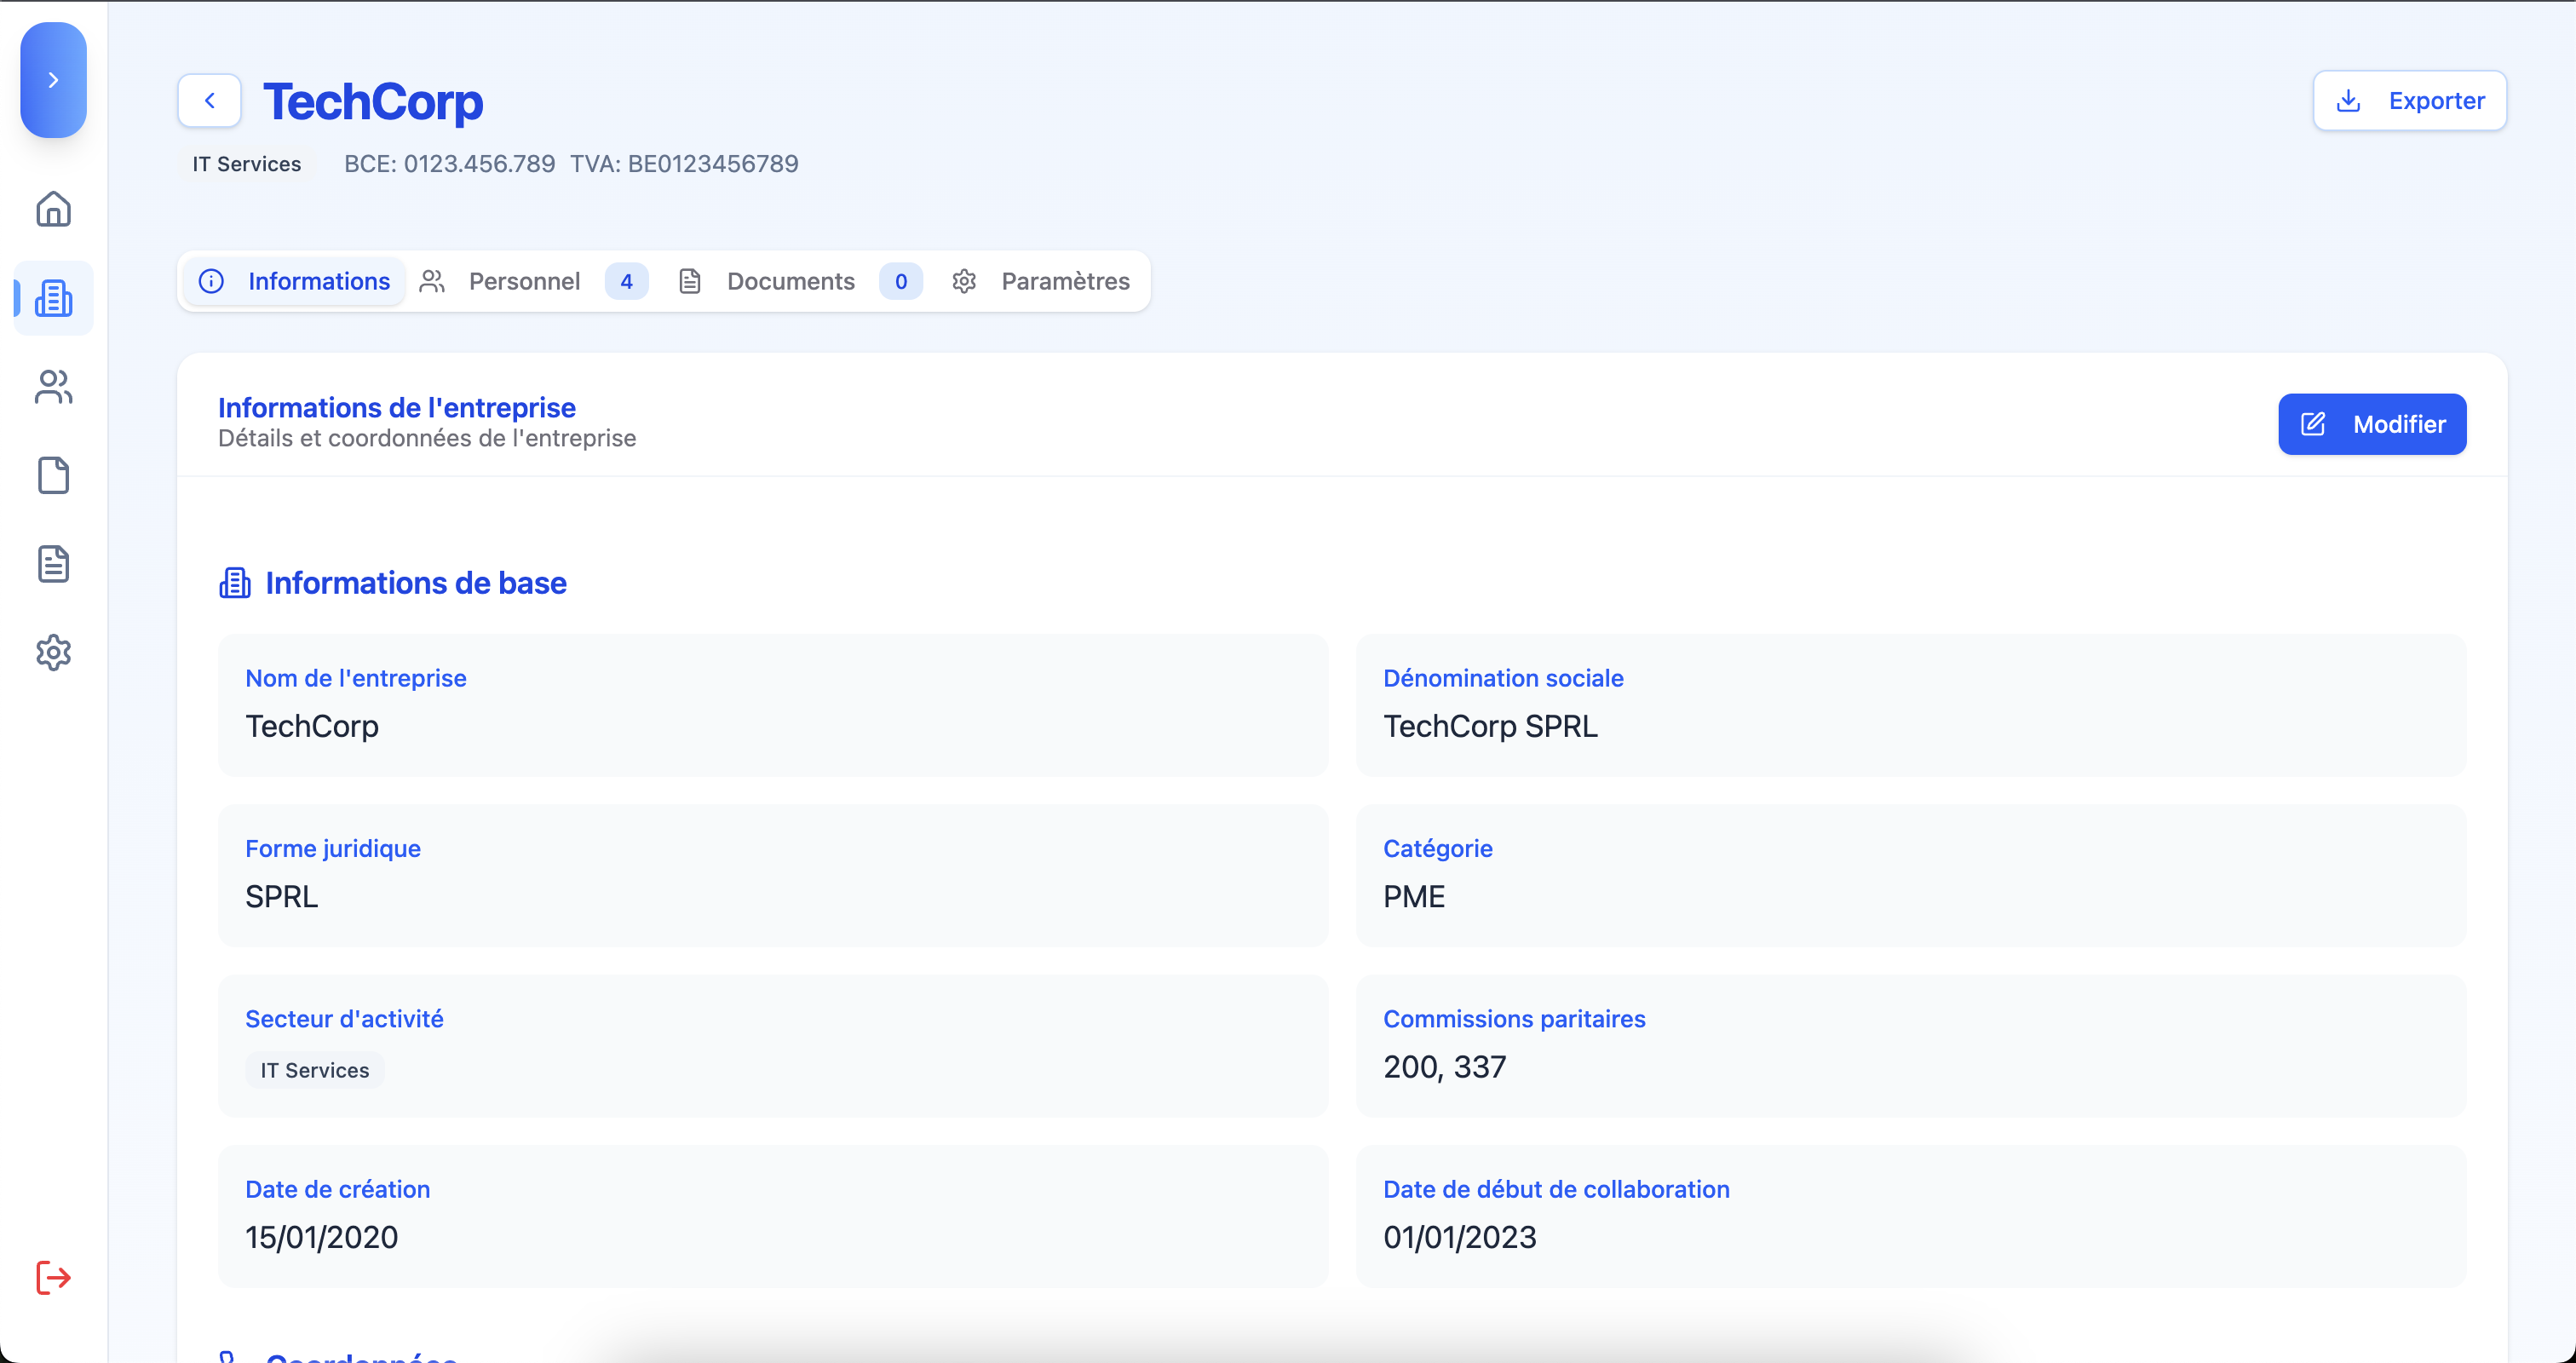
\includegraphics[width=1\textwidth]{SecuComPreviewCompany.png}
  \caption{Interface de gestion des entreprises dans SecuCom}
  \label{fig:companyInterface}
\end{figure}

\vspace{0.5cm}

Cette entité est au centre de nombreuses relations : elle est liée aux contacts d'entreprise, aux collaborateurs et aux déclarations DIMONA.

\subsubsection{Entité Collaborator}

L'entité \texttt{Collaborator} représente un travailleur d'une entreprise cliente. Elle contient des informations personnelles et professionnelles détaillées.

\vspace{0.5cm}

\begin{figure}[H]
  \centering
  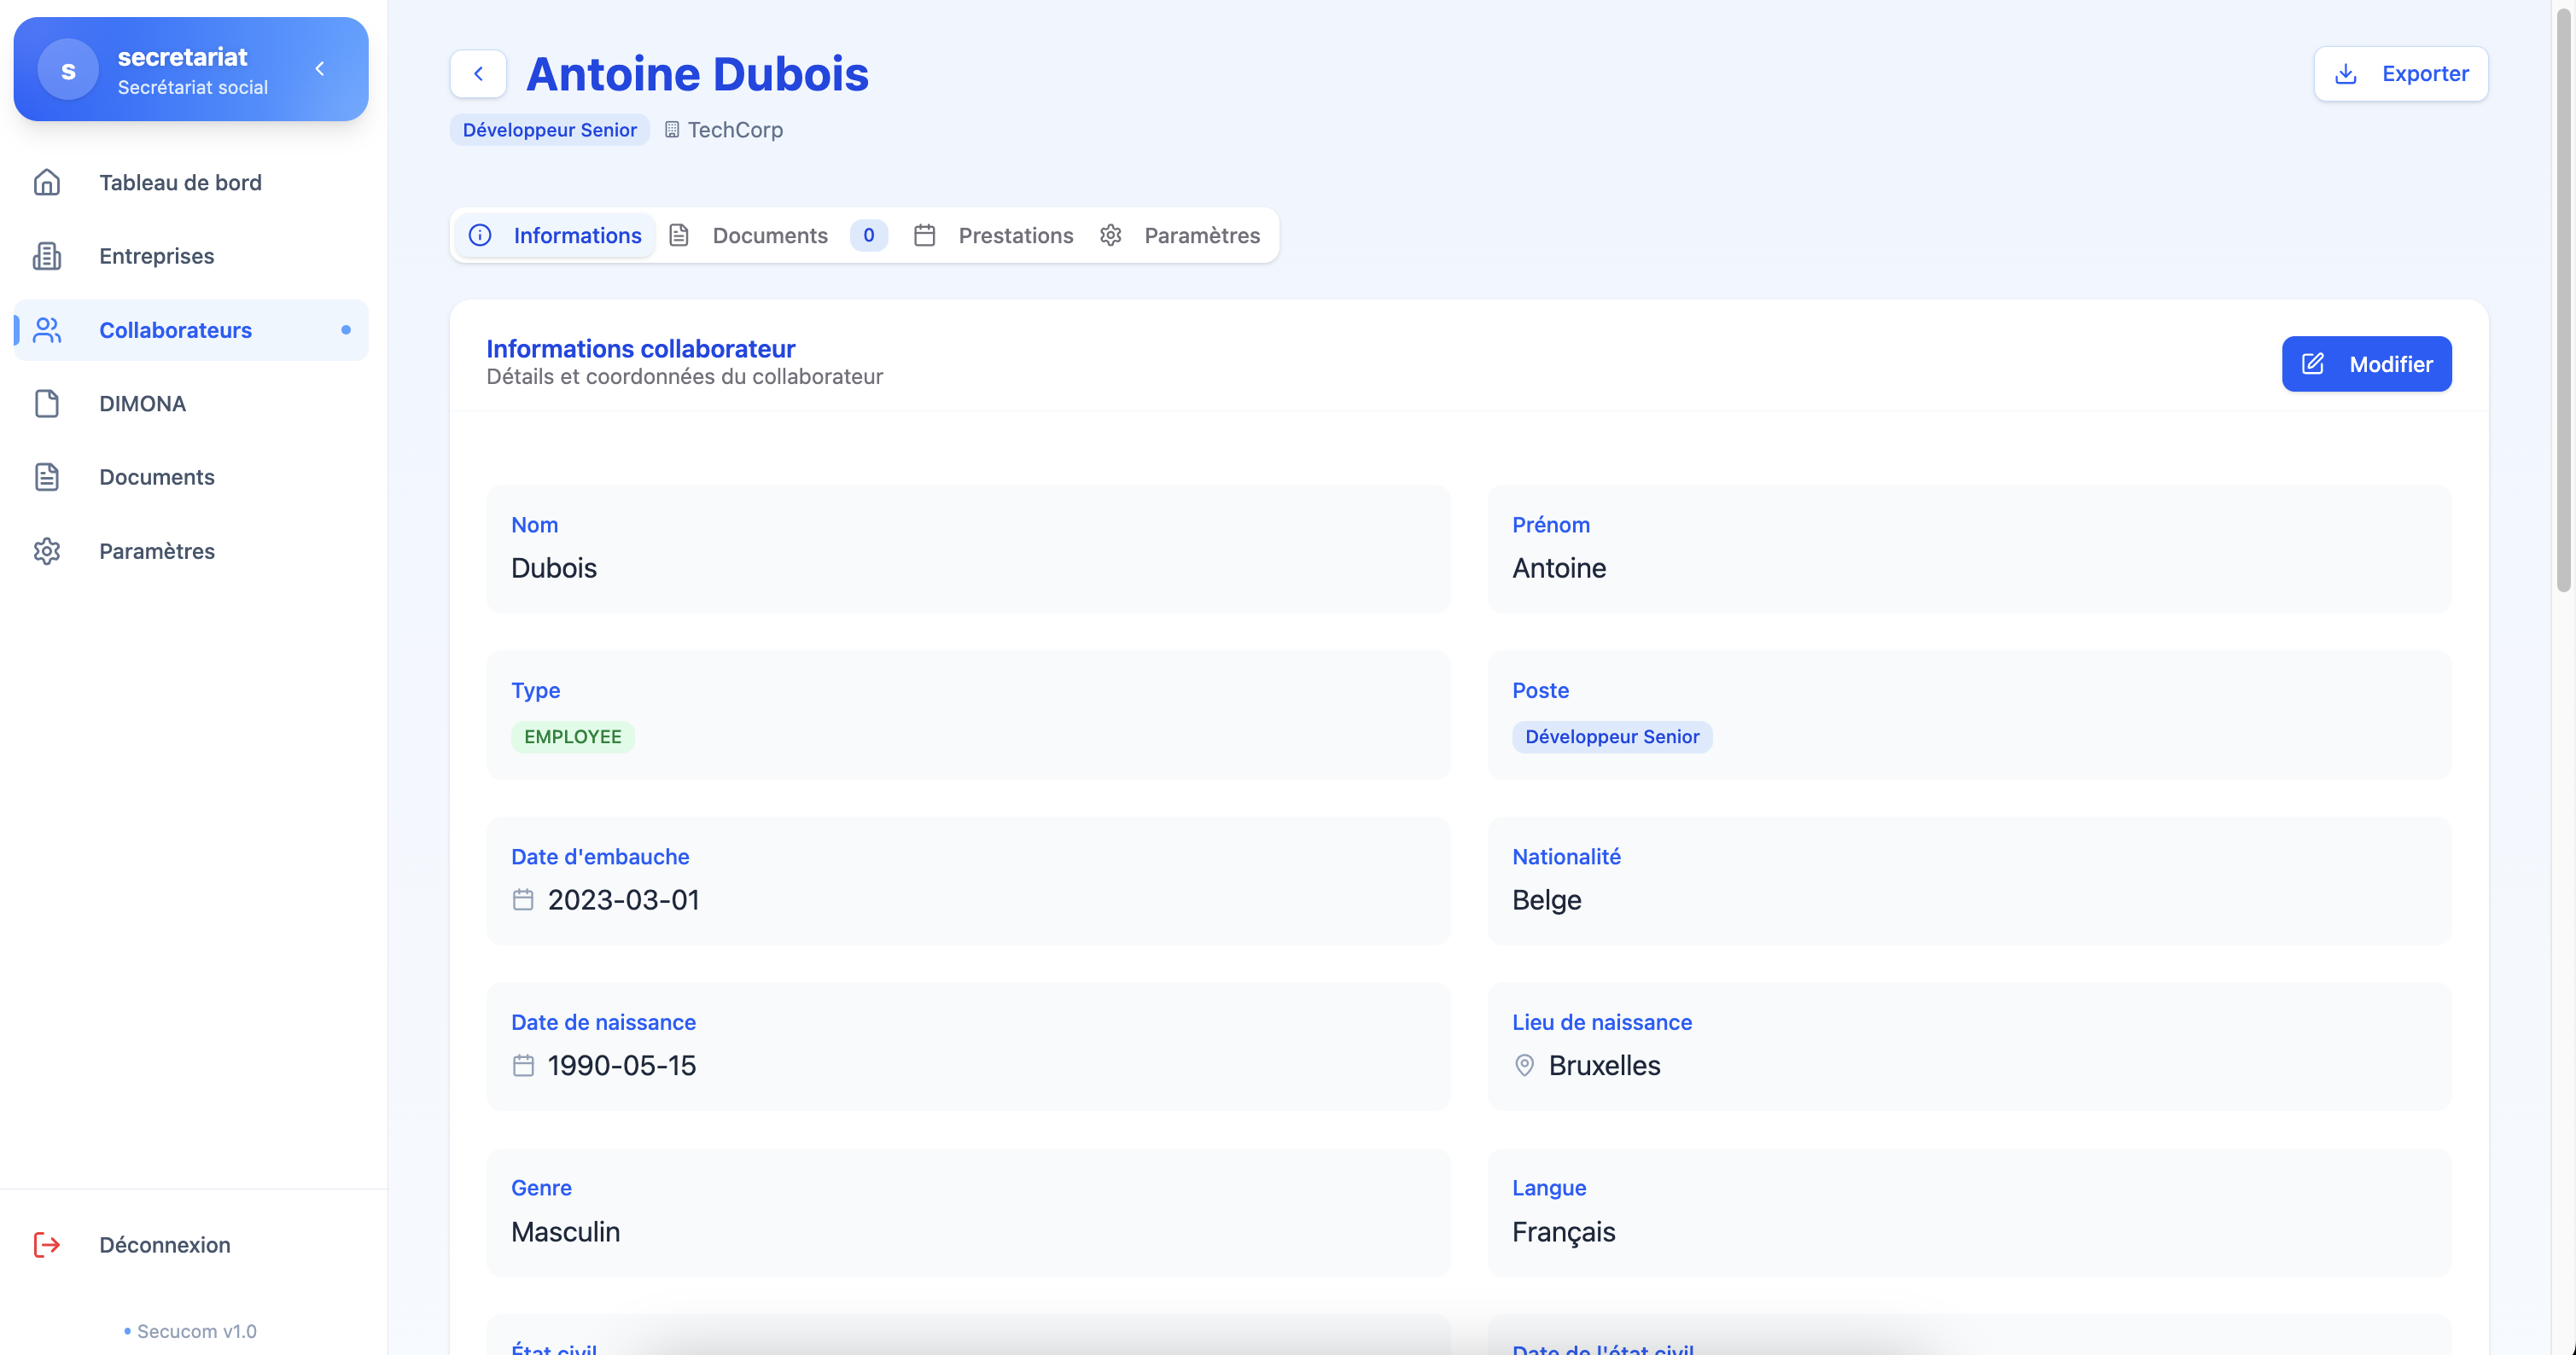
\includegraphics[width=1\textwidth]{SecuComPreviewCollaboratorInfos.png}
  \caption{Interface de gestion des collaborateurs dans SecuCom}
  \label{fig:collaboratorInterface}
\end{figure}

\vspace{0.5cm}

Cette entité utilise des types énumérés pour certains attributs comme le type de collaborateur (\texttt{EMPLOYEE}, \texttt{WORKER}, etc.) et le type de durée de travail (\texttt{FIXED}, \texttt{VARIABLE}).

\subsubsection{Entité Dimona}

L'entité \texttt{Dimona} représente une déclaration DIMONA associée à un collaborateur et à une entreprise.

\vspace{0.5cm}

\begin{figure}[H]
  \centering
  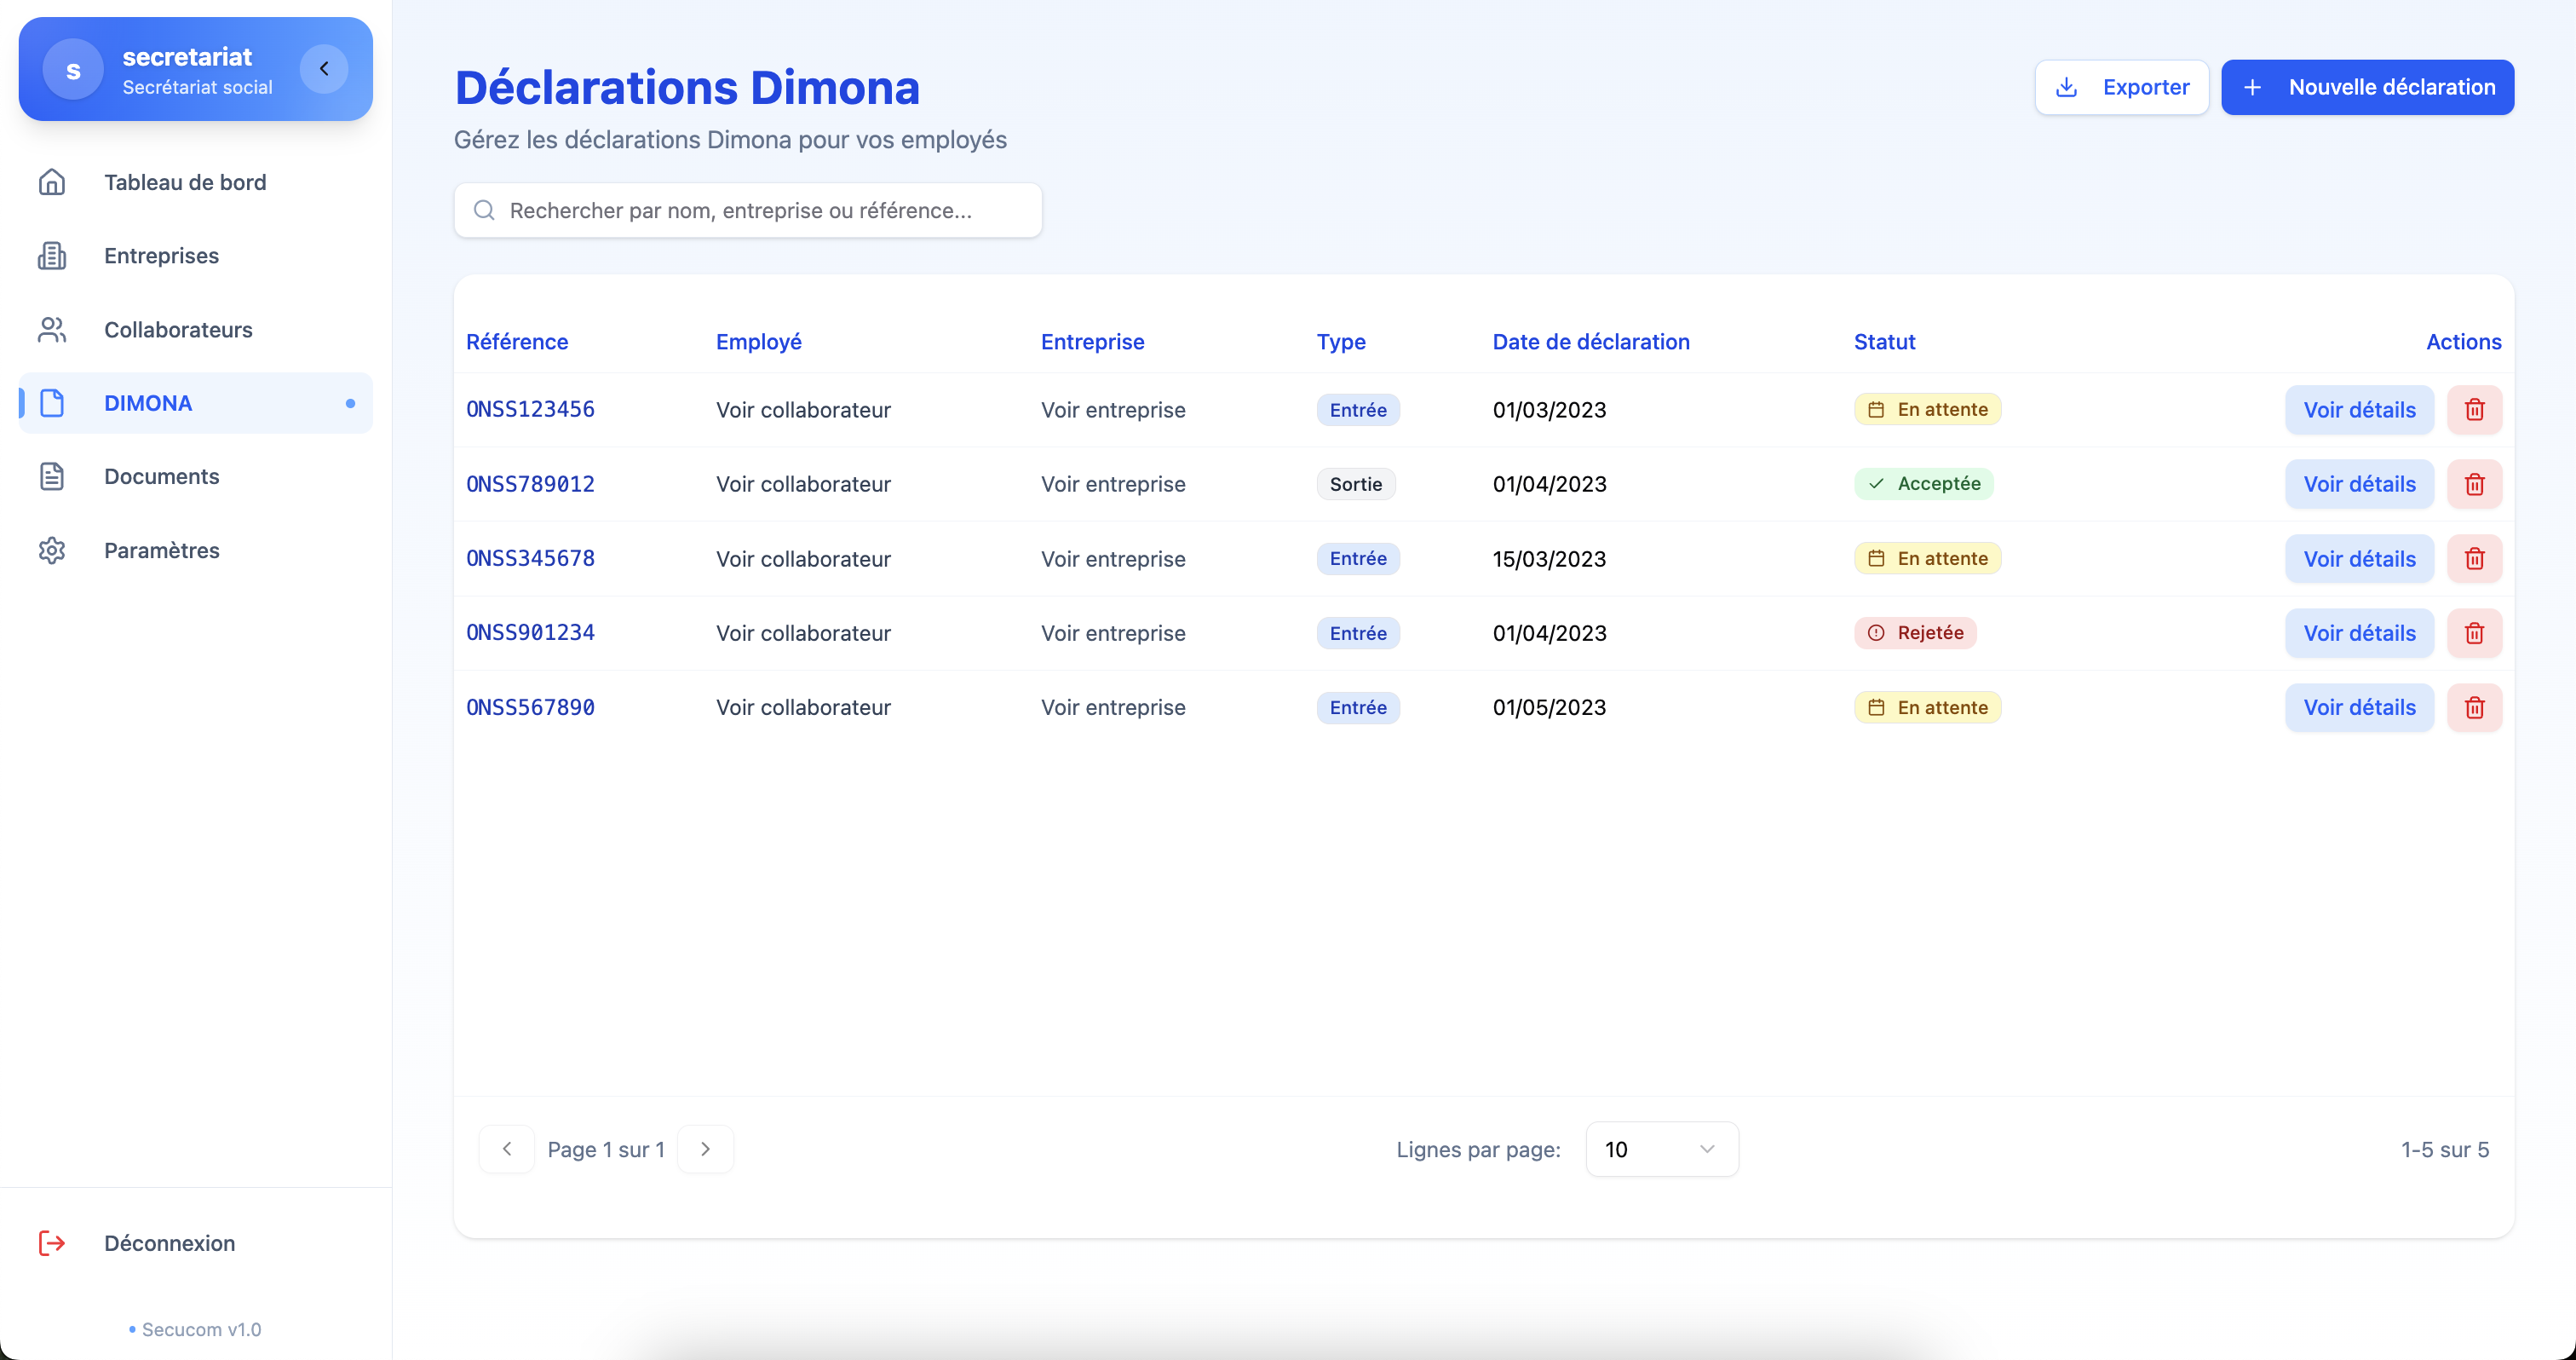
\includegraphics[width=1\textwidth]{SecuComPreviewDimona.png}
  \caption{Interface de gestion des dimonas dans SecuCom}
  \label{fig:companyInterface}
\end{figure}

\vspace{0.5cm}

Cette entité permet de suivre l'état des déclarations DIMONA et de conserver les références attribuées par l'ONSS.

\subsubsection{Autres entités et relations}

Le modèle de données comprend également d'autres entités comme \texttt{Address} (utilisée comme classe embarquée dans plusieurs entités), \texttt{SocialSecretariat} (représentant le secrétariat social) et \texttt{SecretariatEmployee} (représentant un employé du secrétariat social).

\vspace{0.5cm}

\noindent Les relations entre ces entités sont soigneusement définies pour refléter la réalité métier :
\begin{itemize}[leftmargin=*,label=\textcolor{darkgray}{$\bullet$},itemsep=0.3em]
  \item Une entreprise peut avoir plusieurs contacts et plusieurs collaborateurs (relations one-to-many).
  \item Un collaborateur appartient à une seule entreprise (relation many-to-one).
  \item Une déclaration DIMONA est associée à un collaborateur et à une entreprise (relations many-to-one).
  \item Un utilisateur peut avoir plusieurs rôles (relation one-to-many avec une collection d'énumérations).
\end{itemize}

\vspace{0.5cm}

\begin{tcolorbox}[
  title={\textbf{Modélisation des données}},
  colback=blue!5!white,
  colframe=primarycolor,
  fonttitle=\bfseries,
  boxrule=0.5mm,
  arc=2mm,
  left=6mm,
  right=6mm,
  top=6mm,
  bottom=6mm
]
Cette modélisation riche permet de représenter fidèlement les concepts métier tout en facilitant les requêtes et les manipulations de données. L'utilisation de JPA et Hibernate offre une abstraction puissante qui simplifie considérablement le code d'accès aux données.
\end{tcolorbox}

\subsection{Contrôleurs et services}

L'architecture de SecuCom s'appuie sur une séparation claire entre les contrôleurs, qui exposent les API REST, et les services, qui implémentent la logique métier. Cette séparation permet une meilleure organisation du code et facilite les tests.

\subsubsection{Contrôleurs REST}

Les contrôleurs REST sont responsables de la gestion des requêtes HTTP, de la validation des données d'entrée et de la transformation des réponses. Ils sont annotés avec \texttt{@RestController} et définissent des endpoints accessibles via des methodes HTTP (GET, POST, PUT, DELETE).

\vspace{0.5cm}

\begin{table}[H]
\centering
\begin{tabular}{|l|p{10cm}|}
\hline
\textbf{Contrôleur} & \textbf{Responsabilité} \\
\hline
AuthController & Gestion de l'authentification et des tokens JWT \\
\hline
CompanyController & Opérations CRUD sur les entreprises \\
\hline
CollaboratorController & Opérations CRUD sur les collaborateurs \\
\hline
DimonaController & Opérations liées aux déclarations DIMONA \\
\hline
UserController & Opérations sur les utilisateurs \\
\hline
SocialSecretariatController & Opérations liées au secrétariat social \\
\hline
\end{tabular}
\caption{Principaux contrôleurs de SecuCom}
\end{table}

\vspace{0.5cm}

Les contrôleurs utilisent des objets DTO (Data Transfer Object) pour les échanges avec les clients, ce qui permet de découpler les modèles internes des représentations externes.

\subsubsection{Services métier}

Les services métier encapsulent la logique fonctionnelle de l'application. Ils orchestrent les opérations entre les repositories et les contrôleurs, appliquent les règles métier et gèrent les transactions.

\vspace{0.5cm}

\begin{note}
Les services utilisent l'annotation \texttt{@Transactional} pour gérer les transactions de manière déclarative, assurant l'intégrité des données même en cas d'erreur.
\end{note}

\newpage

\noindent Les principaux services de l'application sont :
\begin{itemize}[leftmargin=*,label=\textcolor{darkgray}{$\bullet$},itemsep=0.3em]
  \item \texttt{AuthService} : Gère l'authentification et la génération des tokens.
  \item \texttt{CompanyService} : Implémente la logique métier pour les entreprises.
  \item \texttt{CollaboratorService} : Implémente la logique métier pour les collaborateurs.
  \item \texttt{DimonaService} : Implémente la logique métier pour les déclarations DIMONA.
  \item \texttt{UserService} : Implémente la logique métier pour les utilisateurs.
  \item \texttt{SocialSecretariatService} : Implémente la logique métier pour le secrétariat social.
\end{itemize}

\subsubsection{Repositories}

Les repositories fournissent une abstraction de l'accès aux données. Ils sont implémentés en utilisant Spring Data JPA, qui génère automatiquement les implémentations à partir d'interfaces.

\vspace{0.5cm}

\begin{tcolorbox}[
  title={\textbf{Avantages des repositories Spring Data}},
  colback=blue!5!white,
  colframe=primarycolor,
  fonttitle=\bfseries,
  boxrule=0.5mm,
  arc=2mm,
  left=6mm,
  right=6mm,
  top=6mm,
  bottom=6mm
]
Cette approche permet de réduire considérablement le code boilerplate tout en offrant des fonctionnalités puissantes comme le filtrage, le tri et la pagination. Les développeurs peuvent se concentrer sur la logique métier plutôt que sur les détails techniques de l'accès aux données.
\end{tcolorbox}

\subsubsection{DTOs (Data Transfer Objects)}

Les DTOs sont utilisés pour découpler les modèles internes des représentations externes. Ils permettent de :
\begin{itemize}[leftmargin=*,label=\textcolor{darkgray}{$\bullet$},itemsep=0.3em]
  \item Contrôler précisément les données exposées aux clients
  \item Valider les données d'entrée indépendamment des entités
  \item Adapter le format des données aux besoins spécifiques des clients
\end{itemize}

\vspace{0.5cm}

La conversion entre DTOs et entités est généralement gérée par des bibliothèques comme ModelMapper ou MapStruct, ou par des methodes de conversion manuelles dans les services.

\section{Fonctionnalités principales}

\subsection{Gestion des entreprises}

La gestion des entreprises est une fonctionnalité centrale de SecuCom, permettant au secrétariat social de gérer efficacement ses clients. Cette fonctionnalité est implémentée à travers plusieurs composants qui travaillent ensemble.

\vspace{0.5cm}

\begin{figure}[H]
  \centering
  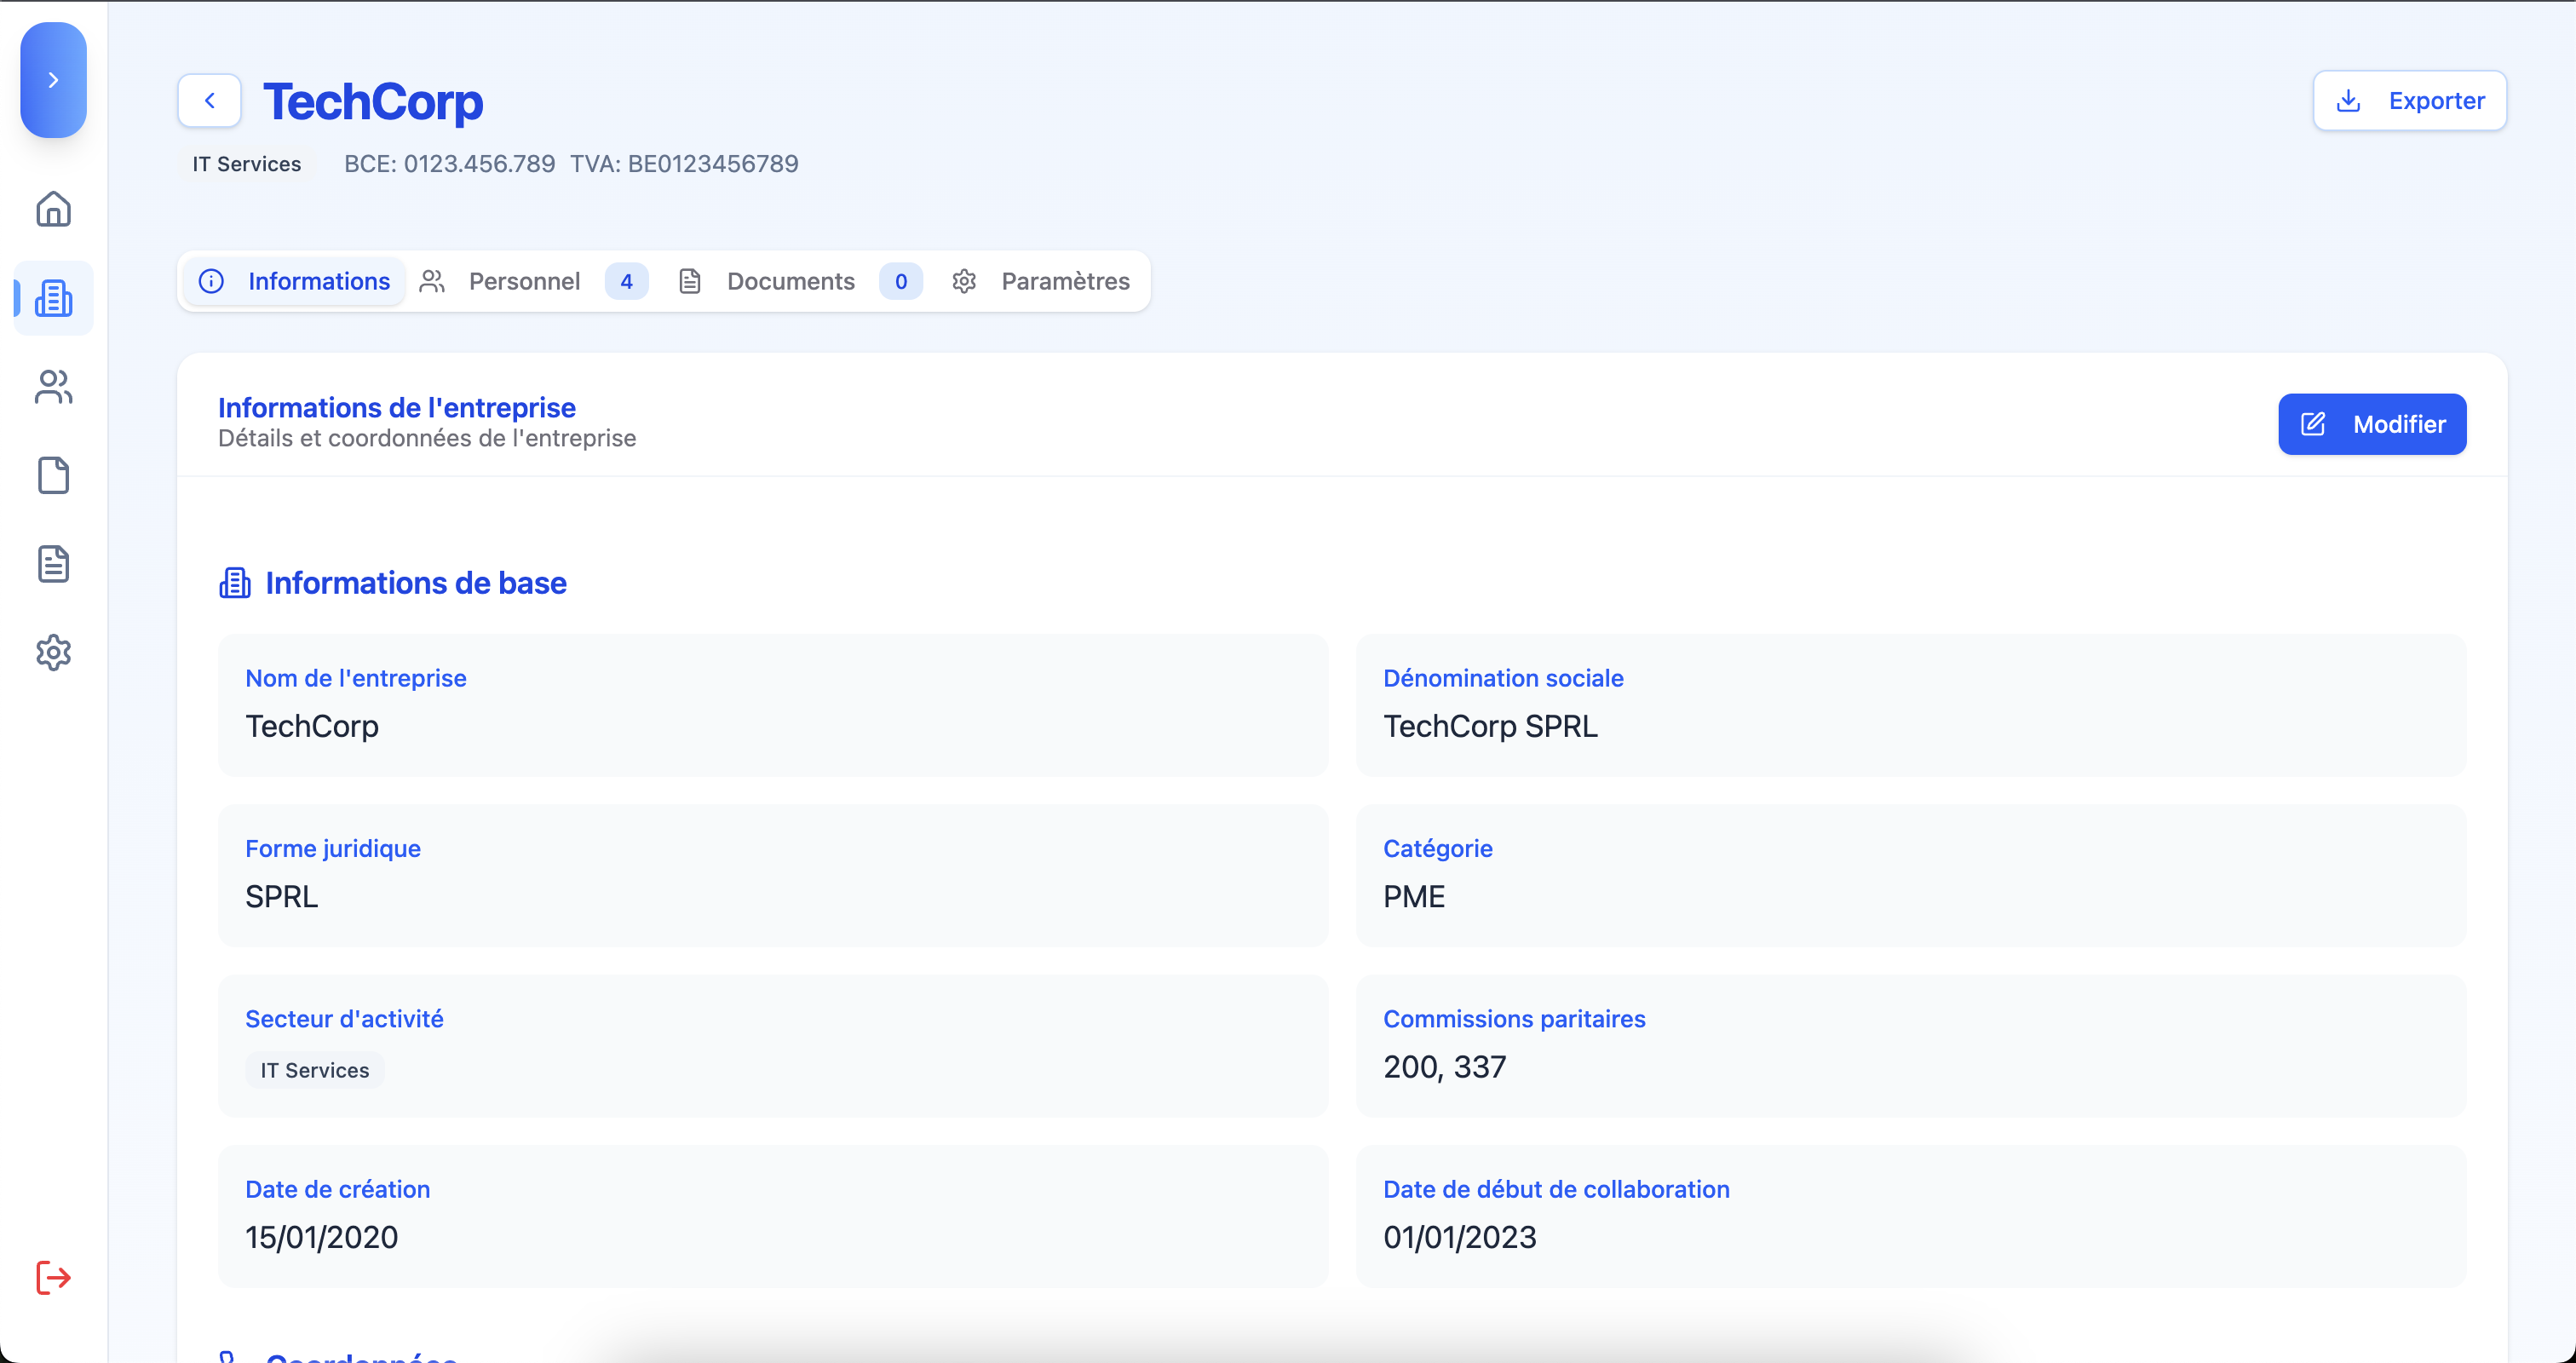
\includegraphics[width=1\textwidth]{SecuComPreviewCompany.png}
  \caption{Interface de gestion des entreprises dans SecuCom}
  \label{fig:companyManagementInterface}
\end{figure}
\vspace{0.5cm}
\begin{figure}[H]
  \centering
  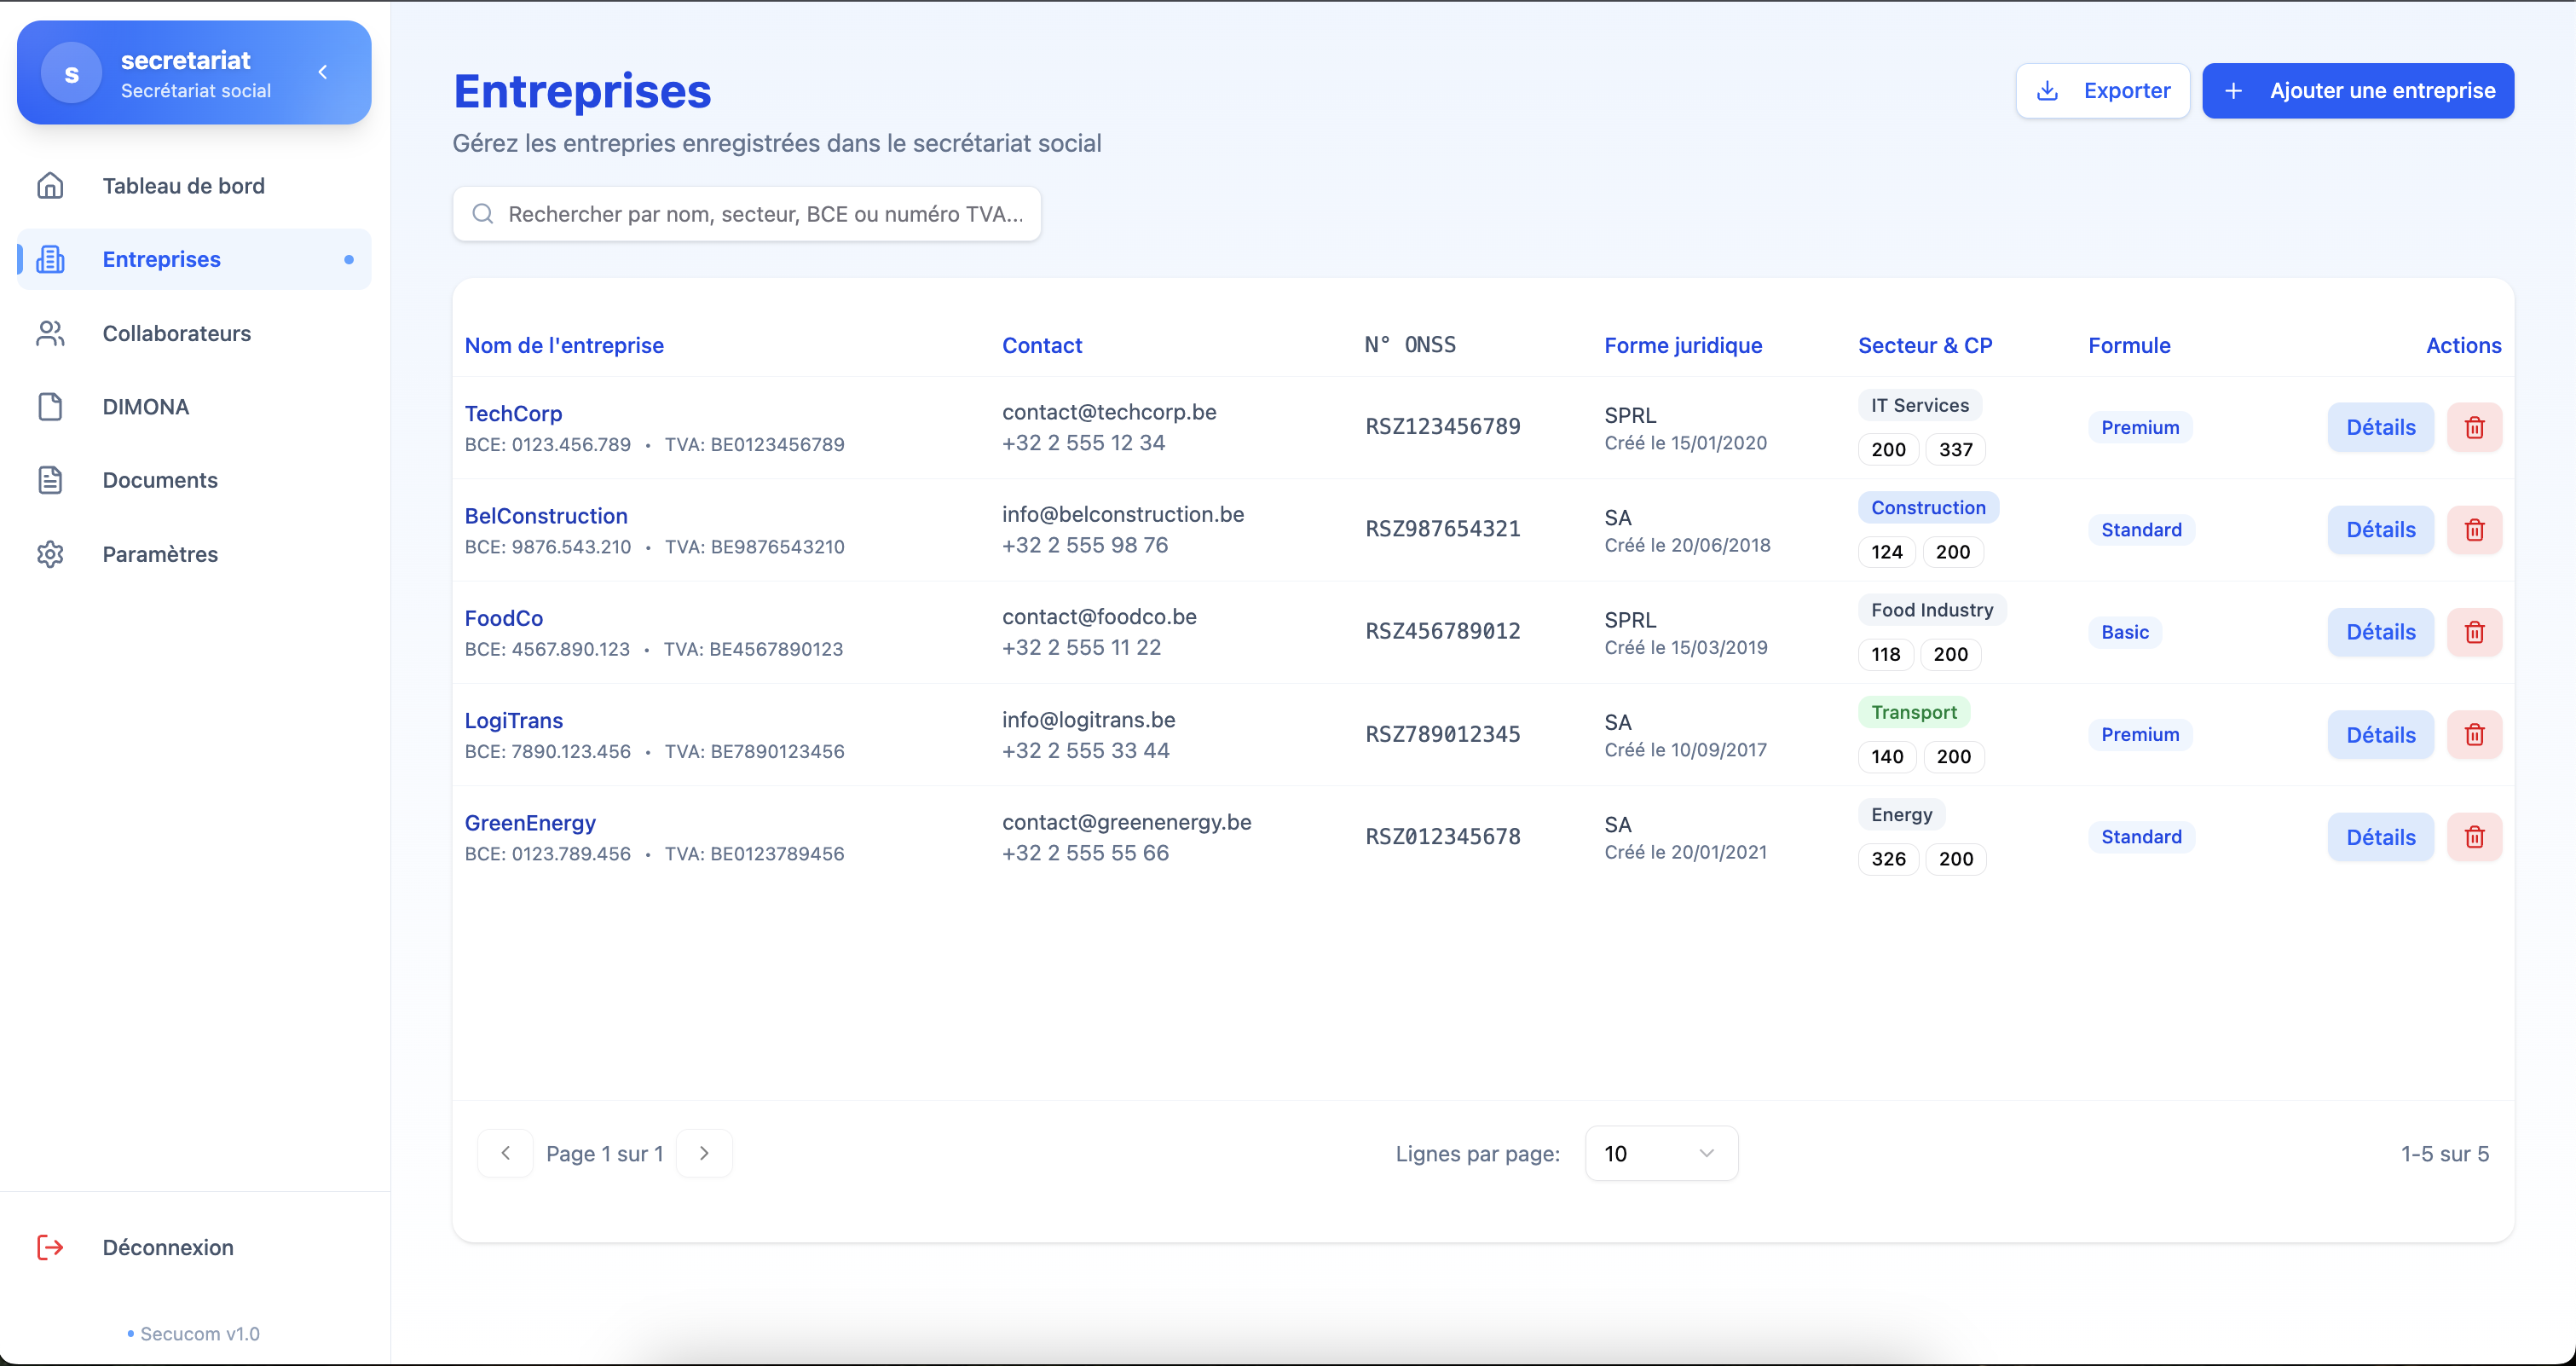
\includegraphics[width=1\textwidth]{SecuComPreviewCompanyList.png}
  \caption{Interface de gestion des entreprises dans SecuCom}
  \label{fig:companyManagementInterface}
\end{figure}

\subsubsection{Modèle de données}

Le modèle de données pour les entreprises est centré autour de l'entité \texttt{Company}, qui stocke toutes les informations nécessaires :

\vspace{0.5cm}

\begin{itemize}[leftmargin=*,label=\textcolor{darkgray}{$\bullet$},itemsep=0.3em]
  \item \textbf{Informations d'identification} : nom, numéro BCE, numéro ONSS, numéro TVA
  \item \textbf{Informations de contact} : téléphone, email, adresse
  \item \textbf{Informations bancaires} : IBAN
  \item \textbf{Informations légales} : forme juridique, secteur d'activité, commissions paritaires
  \item \textbf{Informations de collaboration} : date de début, formule souscrite, fréquence de déclaration
\end{itemize}

\vspace{0.5cm}

Cette entité est liée à d'autres entités importantes :
\begin{itemize}[leftmargin=*,label=\textcolor{darkgray}{$\bullet$},itemsep=0.3em]
  \item \texttt{CompanyContact} : Utilisateurs ayant accès aux données de l'entreprise
  \item \texttt{Collaborator} : Travailleurs de l'entreprise
  \item \texttt{Dimona} : Déclarations DIMONA associées à l'entreprise
\end{itemize}

\subsubsection{API REST}

L'API REST pour la gestion des entreprises est exposée par le \texttt{CompanyController}, qui offre les endpoints suivants :

\vspace{0.5cm}

\begin{tcolorbox}[
  title={\textbf{Endpoints de gestion des entreprises}},
  colback=blue!5!white,
  colframe=primarycolor,
  fonttitle=\bfseries,
  boxrule=0.5mm,
  arc=2mm,
  left=6mm,
  right=6mm,
  top=6mm,
  bottom=6mm
]
\begin{itemize}[leftmargin=*,label=\textcolor{darkgray}{$\bullet$},itemsep=0.3em]
  \item \texttt{POST /company} : Création d'une nouvelle entreprise
  \item \texttt{GET /company/\{id\}} : Récupération des détails d'une entreprise
  \item \texttt{GET /company} : Récupération de la liste des entreprises
  \item \texttt{PUT /company/\{id\}} : Mise à jour des informations d'une entreprise
  \item \texttt{DELETE /company/\{id\}} : Suppression d'une entreprise
  \item \texttt{GET /company/check/bce/\{bceNumber\}} : Vérification de l'existence d'un numéro BCE
  \item \texttt{GET /company/check/onss/\{onssNumber\}} : Vérification de l'existence d'un numéro ONSS
  \item \texttt{GET /company/check/vat/\{vatNumber\}} : Vérification de l'existence d'un numéro TVA
\end{itemize}
\end{tcolorbox}

\vspace{0.5cm}

\begin{note}
Ces endpoints sont sécurisés et accessibles uniquement aux utilisateurs autorisés (administrateurs et employés du secrétariat social).
\end{note}
\newpage

\subsubsection{Logique métier}

La logique métier pour la gestion des entreprises est implémentée dans le \texttt{CompanyService}, qui offre les fonctionnalités suivantes :

\vspace{0.5cm}

\begin{itemize}[leftmargin=*,label=\textcolor{darkgray}{$\bullet$},itemsep=0.3em]
  \item Validation des données d'entreprise (unicité des numéros BCE, ONSS et TVA)
  \item Création et mise à jour des entreprises avec gestion des relations
  \item Récupération des entreprises avec filtrage et pagination
  \item Suppression des entreprises avec gestion des dépendances
\end{itemize}

\vspace{0.5cm}

Le service implémente également des règles métier spécifiques, comme la vérification de la validité des numéros BCE et ONSS selon les formats belges.

\subsubsection{Gestion des contacts d'entreprise}

La gestion des contacts d'entreprise est une fonctionnalité complémentaire qui permet de définir quels utilisateurs ont accès aux données d'une entreprise. Elle est implémentée à travers le \texttt{CompanyContactService} et le \texttt{CompanyContactController}.

\vspace{0.5cm}

\begin{tcolorbox}[
  title={\textbf{Accès sécurisé par entreprise}},
  colback=blue!5!white,
  colframe=primarycolor,
  fonttitle=\bfseries,
  boxrule=0.5mm,
  arc=2mm,
  left=6mm,
  right=6mm,
  top=6mm,
  bottom=6mm
]
Les contacts d'entreprise sont des utilisateurs spécialisés (héritant de \texttt{User}) qui ont le rôle \texttt{ROLE\_COMPANY} et sont associés à une entreprise spécifique. Ils peuvent accéder uniquement aux données de leur propre entreprise, ce qui garantit une séparation stricte des données entre les différents clients du secrétariat social.
\end{tcolorbox}

\subsection{Gestion des collaborateurs}

La gestion des collaborateurs est une autre fonctionnalité clé de SecuCom, permettant de gérer les travailleurs des entreprises clientes (qu'ils soient employés, ouvriers, freelances, stagiaires ou étudiants). Cette fonctionnalité est particulièrement importante car elle sert de base pour les déclarations DIMONA.

\vspace{0.5cm}

\begin{figure}[H]
  \centering
  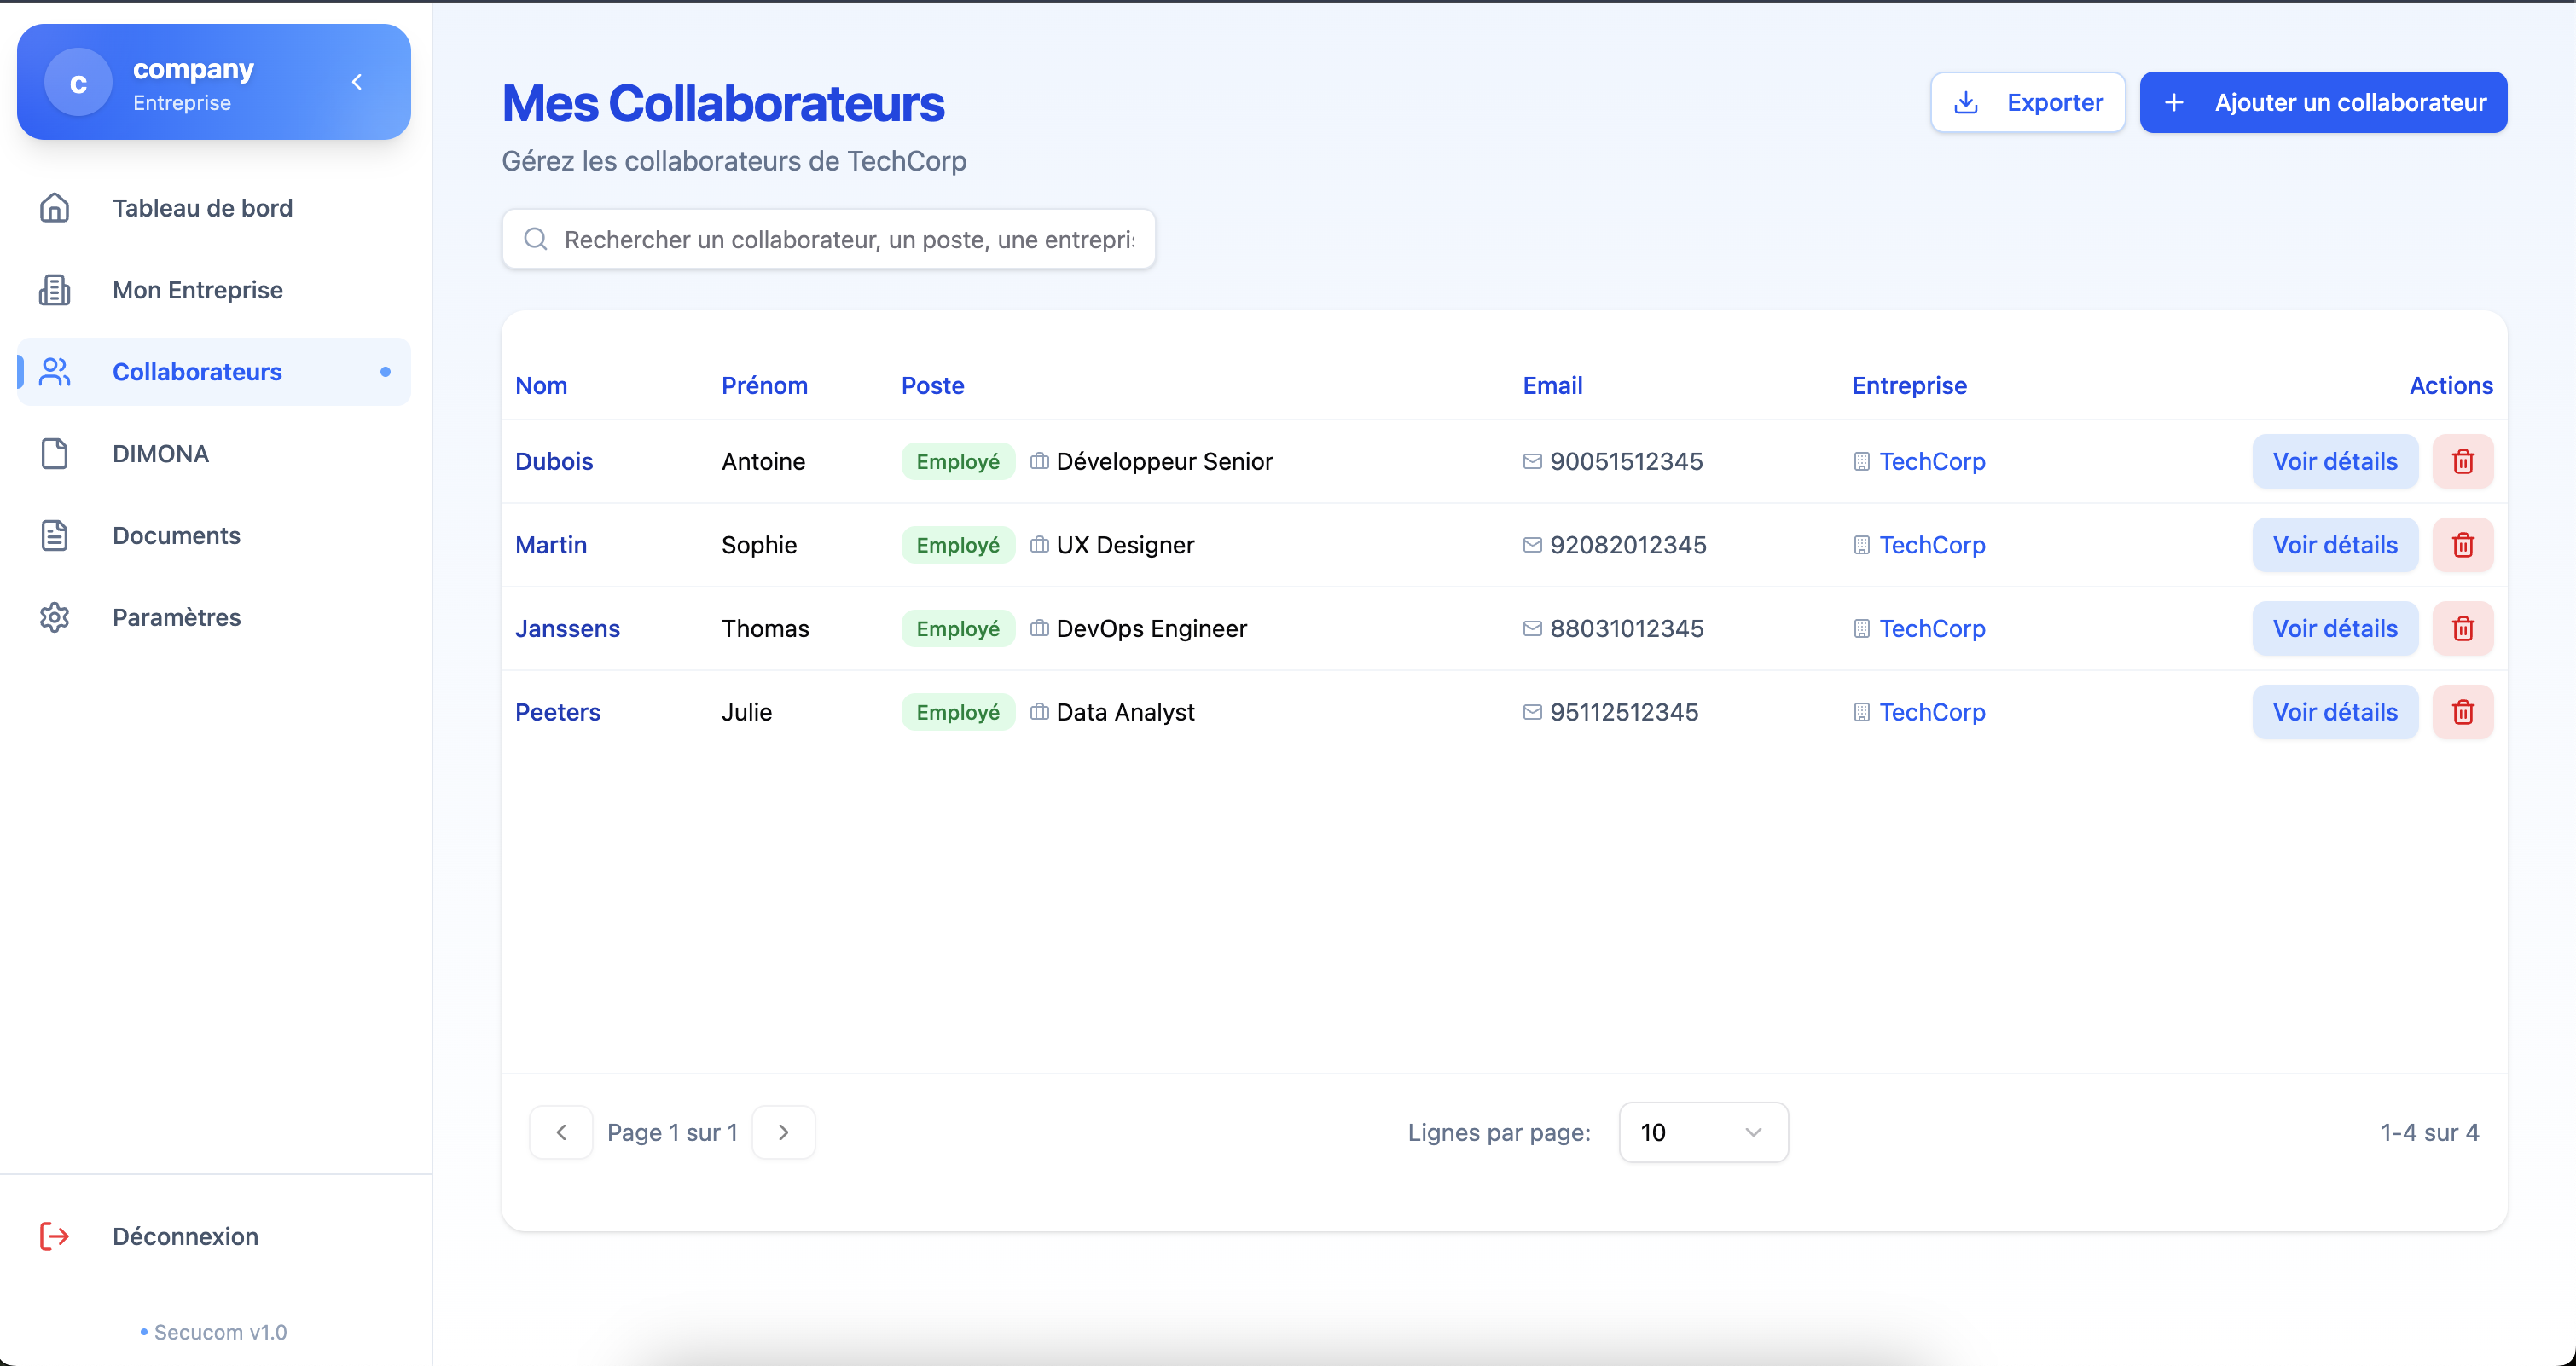
\includegraphics[width=1\textwidth]{SecuComPreviewCompanySpace.png}
  \caption{Interface de gestion des collaborateurs dans SecuCom}
  \label{fig:companyManagementInterface}
\end{figure}
\vspace{0.5cm}
\begin{figure}[H]
  \centering
  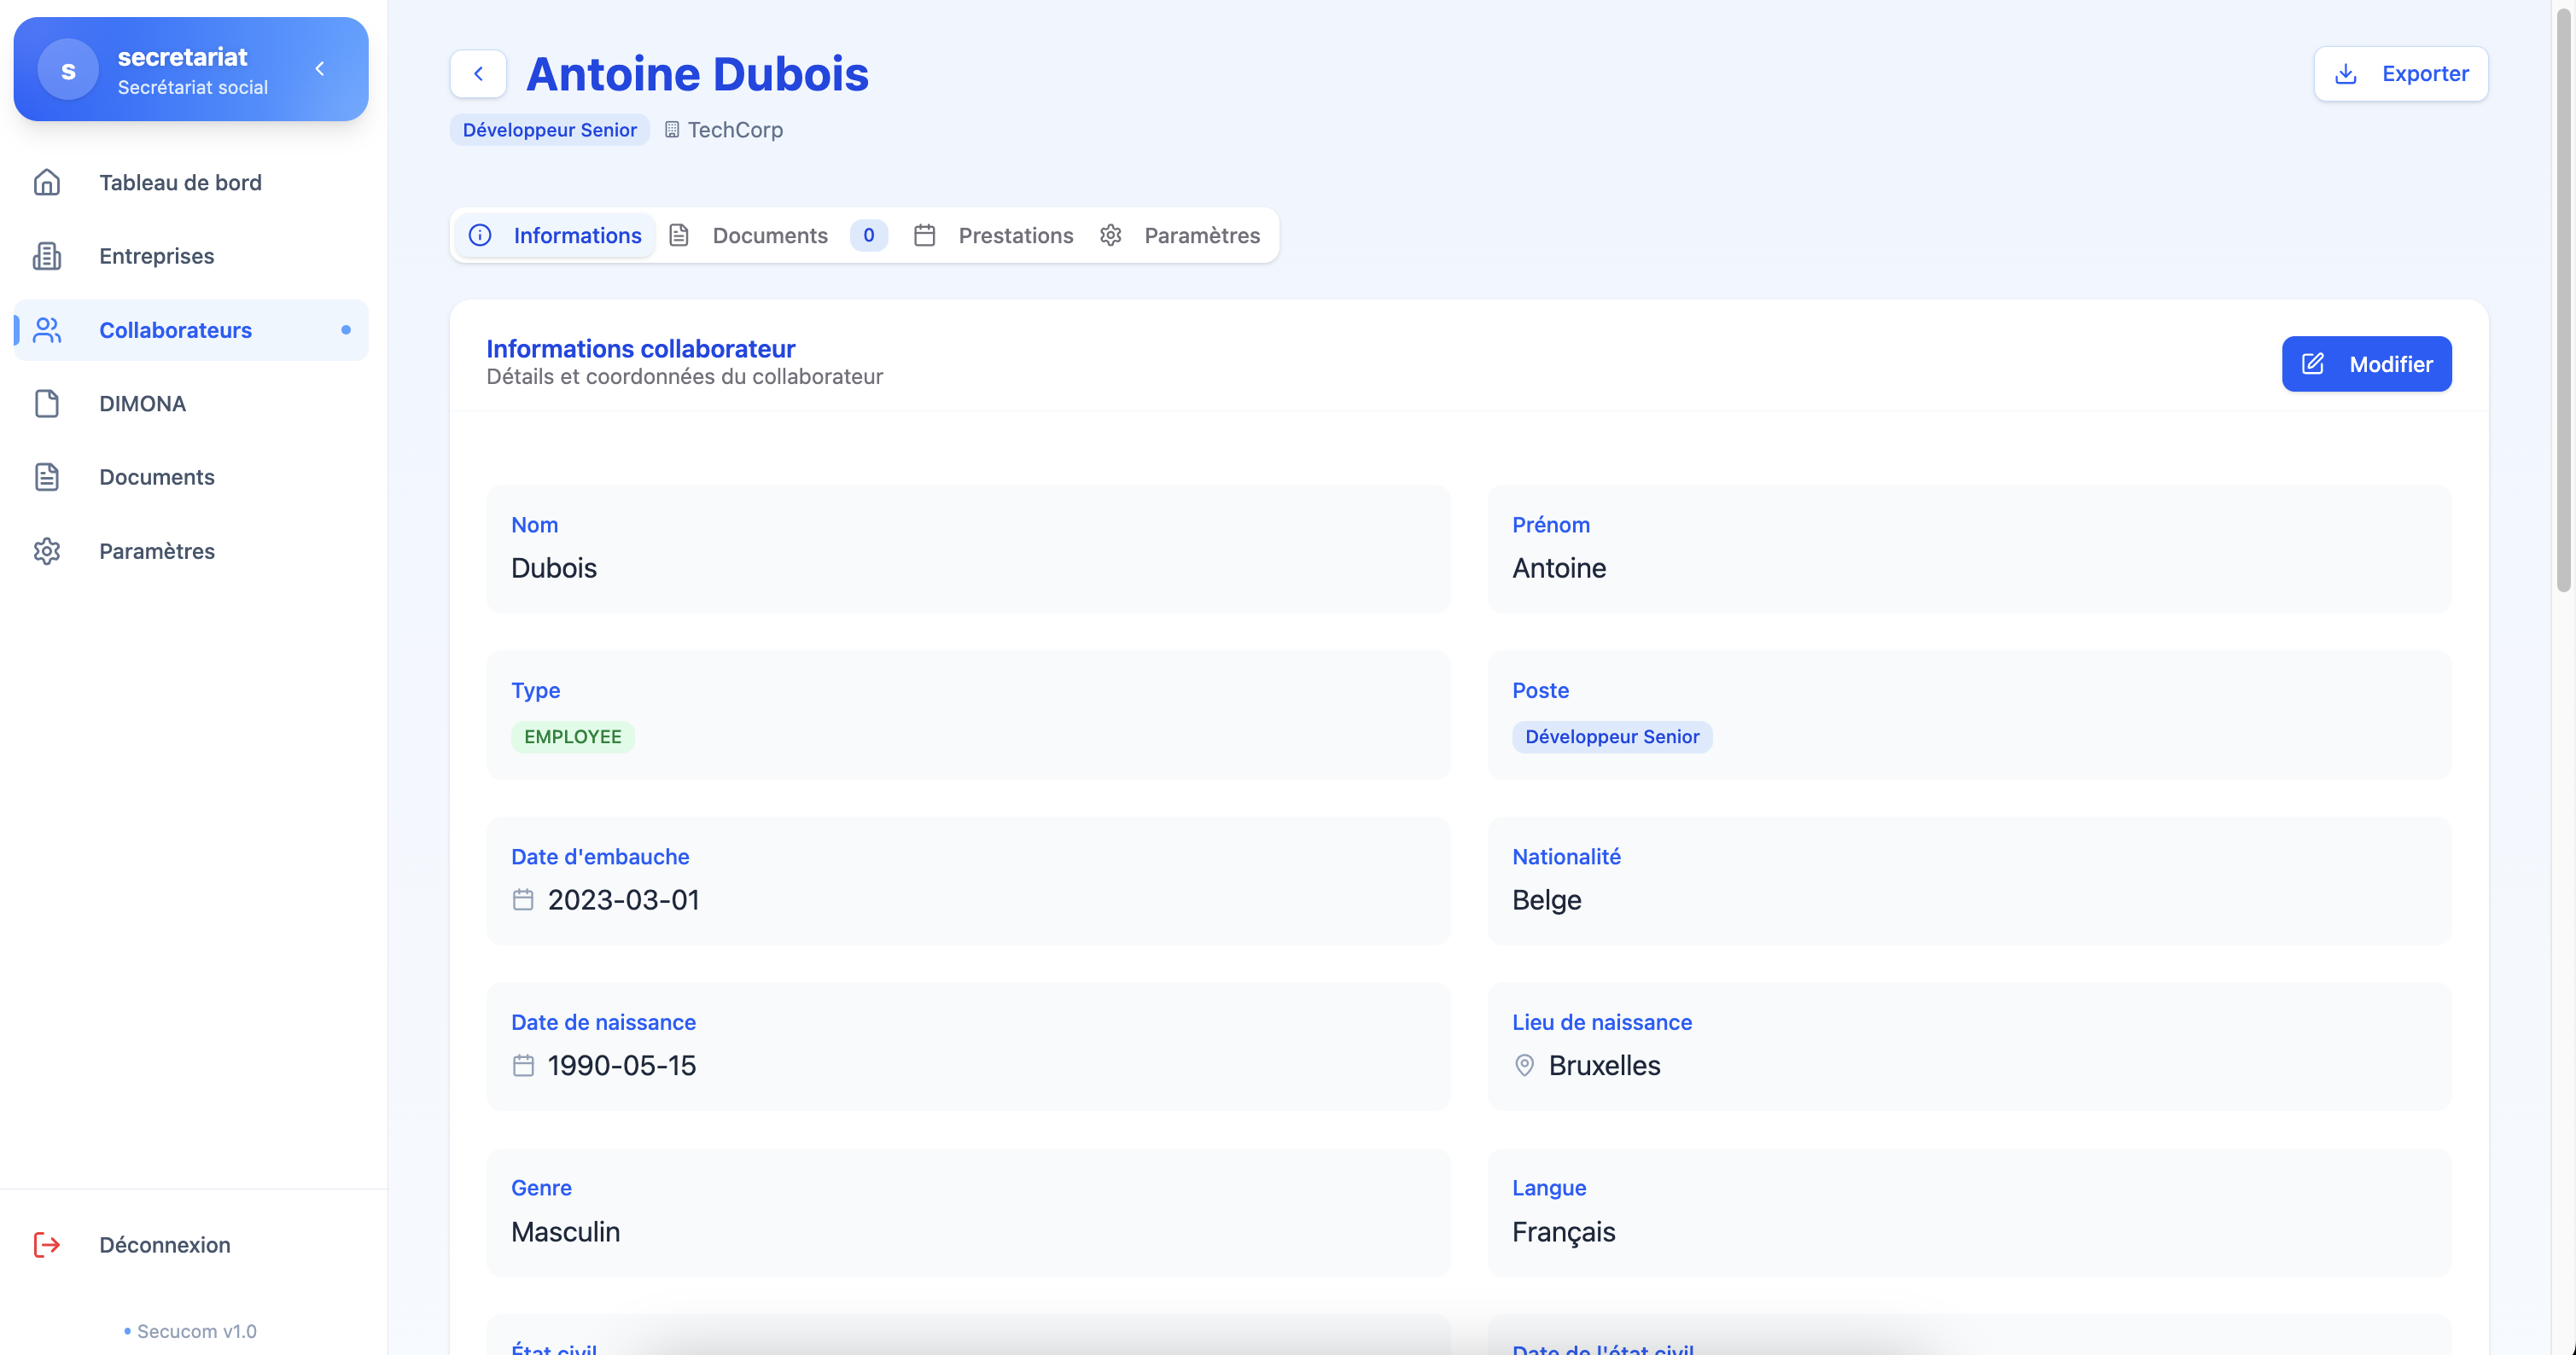
\includegraphics[width=1\textwidth]{SecuComPreviewCollaboratorInfos.png}
  \caption{Interface de gestion des collaborateurs dans SecuCom}
  \label{fig:companyManagementInterface}
\end{figure}

\subsubsection{Modèle de données}

Le modèle de données pour les collaborateurs est centré autour de l'entité \texttt{Collaborator}, qui stocke de nombreuses informations :

\vspace{0.5cm}

\begin{itemize}[leftmargin=*,label=\textcolor{darkgray}{$\bullet$},itemsep=0.3em]
  \item \textbf{Informations personnelles} : nom, prénom, nationalité, date de naissance, lieu de naissance, genre, langue, état civil
  \item \textbf{Informations d'identification} : numéro national (unique)
  \item \textbf{Informations professionnelles} : date d'entrée en service, fonction, type de contrat, régime de travail
  \item \textbf{Informations de rémunération} : salaire, avantages extra-légaux
  \item \textbf{Informations bancaires} : IBAN pour le versement du salaire
\end{itemize}

\vspace{0.5cm}

L'entité \texttt{Collaborator} utilise plusieurs types énumérés pour catégoriser les collaborateurs :
\begin{itemize}[leftmargin=*,label=\textcolor{darkgray}{$\bullet$},itemsep=0.3em]
  \item \texttt{CollaboratorType} : EMPLOYEE, WORKER, FREELANCE, INTERN, STUDENT
  \item \texttt{WorkDurationType} : FIXED, VARIABLE
  \item \texttt{Day} : MONDAY, TUESDAY, WEDNESDAY, THURSDAY, FRIDAY, SATURDAY, SUNDAY (pour les horaires)
\end{itemize}

\vspace{0.5cm}

\begin{note}
Elle utilise également des classes embarquées comme \texttt{Address} pour structurer les informations d'adresse, permettant une meilleure organisation des données et une réutilisation des structures communes.
\end{note}

\subsubsection{API REST}

L'API REST pour la gestion des collaborateurs est exposée par le \texttt{CollaboratorController}, qui offre les endpoints suivants :

\vspace{0.5cm}

\begin{tcolorbox}[
  title={\textbf{Endpoints de gestion des collaborateurs}},
  colback=blue!5!white,
  colframe=primarycolor,
  fonttitle=\bfseries,
  boxrule=0.5mm,
  arc=2mm,
  left=6mm,
  right=6mm,
  top=6mm,
  bottom=6mm
]
\begin{itemize}[leftmargin=*,label=\textcolor{darkgray}{$\bullet$},itemsep=0.3em]
  \item \texttt{POST /collaborators} : Création d'un nouveau collaborateur
  \item \texttt{GET /collaborators/\{id\}} : Récupération des détails d'un collaborateur
  \item \texttt{GET /collaborators} : Récupération de la liste des collaborateurs
  \item \texttt{GET /collaborators/company/\{companyId\}} : Récupération des collaborateurs d'une entreprise
  \item \texttt{PUT /collaborators/\{id\}} : Mise à jour des informations d'un collaborateur
  \item \texttt{DELETE /collaborators/\{id\}} : Suppression d'un collaborateur
\end{itemize}
\end{tcolorbox}

\vspace{0.5cm}

Ces endpoints sont sécurisés et accessibles aux utilisateurs autorisés, avec des restrictions basées sur les rôles et les associations d'entreprise.

\newpage

\subsubsection{Logique métier}

La logique métier pour la gestion des collaborateurs est implémentée dans le \texttt{CollaboratorService}, qui offre les fonctionnalités suivantes :

\vspace{0.5cm}

\begin{itemize}[leftmargin=*,label=\textcolor{darkgray}{$\bullet$},itemsep=0.3em]
  \item Validation des données de collaborateur (unicité du numéro national, validité des dates)
  \item Création et mise à jour des collaborateurs avec gestion des relations
  \item Récupération des collaborateurs avec filtrage par entreprise
  \item Suppression des collaborateurs avec gestion des dépendances (déclarations DIMONA)
\end{itemize}

\vspace{0.5cm}

Le service implémente également des règles métier spécifiques, comme la vérification de la validité du numéro national selon le format belge et la gestion des horaires de travail selon le type de durée de travail (fixe ou variable).

\subsubsection{Validation des données}

La validation des données de collaborateur est particulièrement importante en raison des exigences légales pour les déclarations DIMONA. Elle est implémentée à plusieurs niveaux :

\vspace{0.5cm}

\begin{tcolorbox}[
  title={\textbf{Approche multi-niveaux de validation}},
  colback=blue!5!white,
  colframe=primarycolor,
  fonttitle=\bfseries,
  boxrule=0.5mm,
  arc=2mm,
  left=6mm,
  right=6mm,
  top=6mm,
  bottom=6mm
]
\begin{itemize}[leftmargin=*,label=\textcolor{darkgray}{$\bullet$},itemsep=0.3em]
  \item \textbf{Niveau présentation} : Validation des DTOs avec les annotations Jakarta Validation (\texttt{@NotNull}, \texttt{@Size}, \texttt{@Pattern}, etc.)
  \item \textbf{Niveau service} : Validation métier dans le service (cohérence des dates, validité du numéro national)
  \item \textbf{Niveau persistance} : Contraintes de base de données (unicité du numéro national)
\end{itemize}

Cette approche garantit l'intégrité et la validité des données de collaborateur, réduisant ainsi les risques d'erreur lors des déclarations officielles auprès de l'ONSS.
\end{tcolorbox}

\subsection{Gestion des déclarations DIMONA}

La gestion des déclarations DIMONA est une fonctionnalité critique de SecuCom, permettant de suivre les déclarations d'emploi auprès de l'ONSS. Cette fonctionnalité est essentielle pour la conformité légale des entreprises clientes.

\vspace{0.5cm}

\begin{figure}[H]
  \centering
  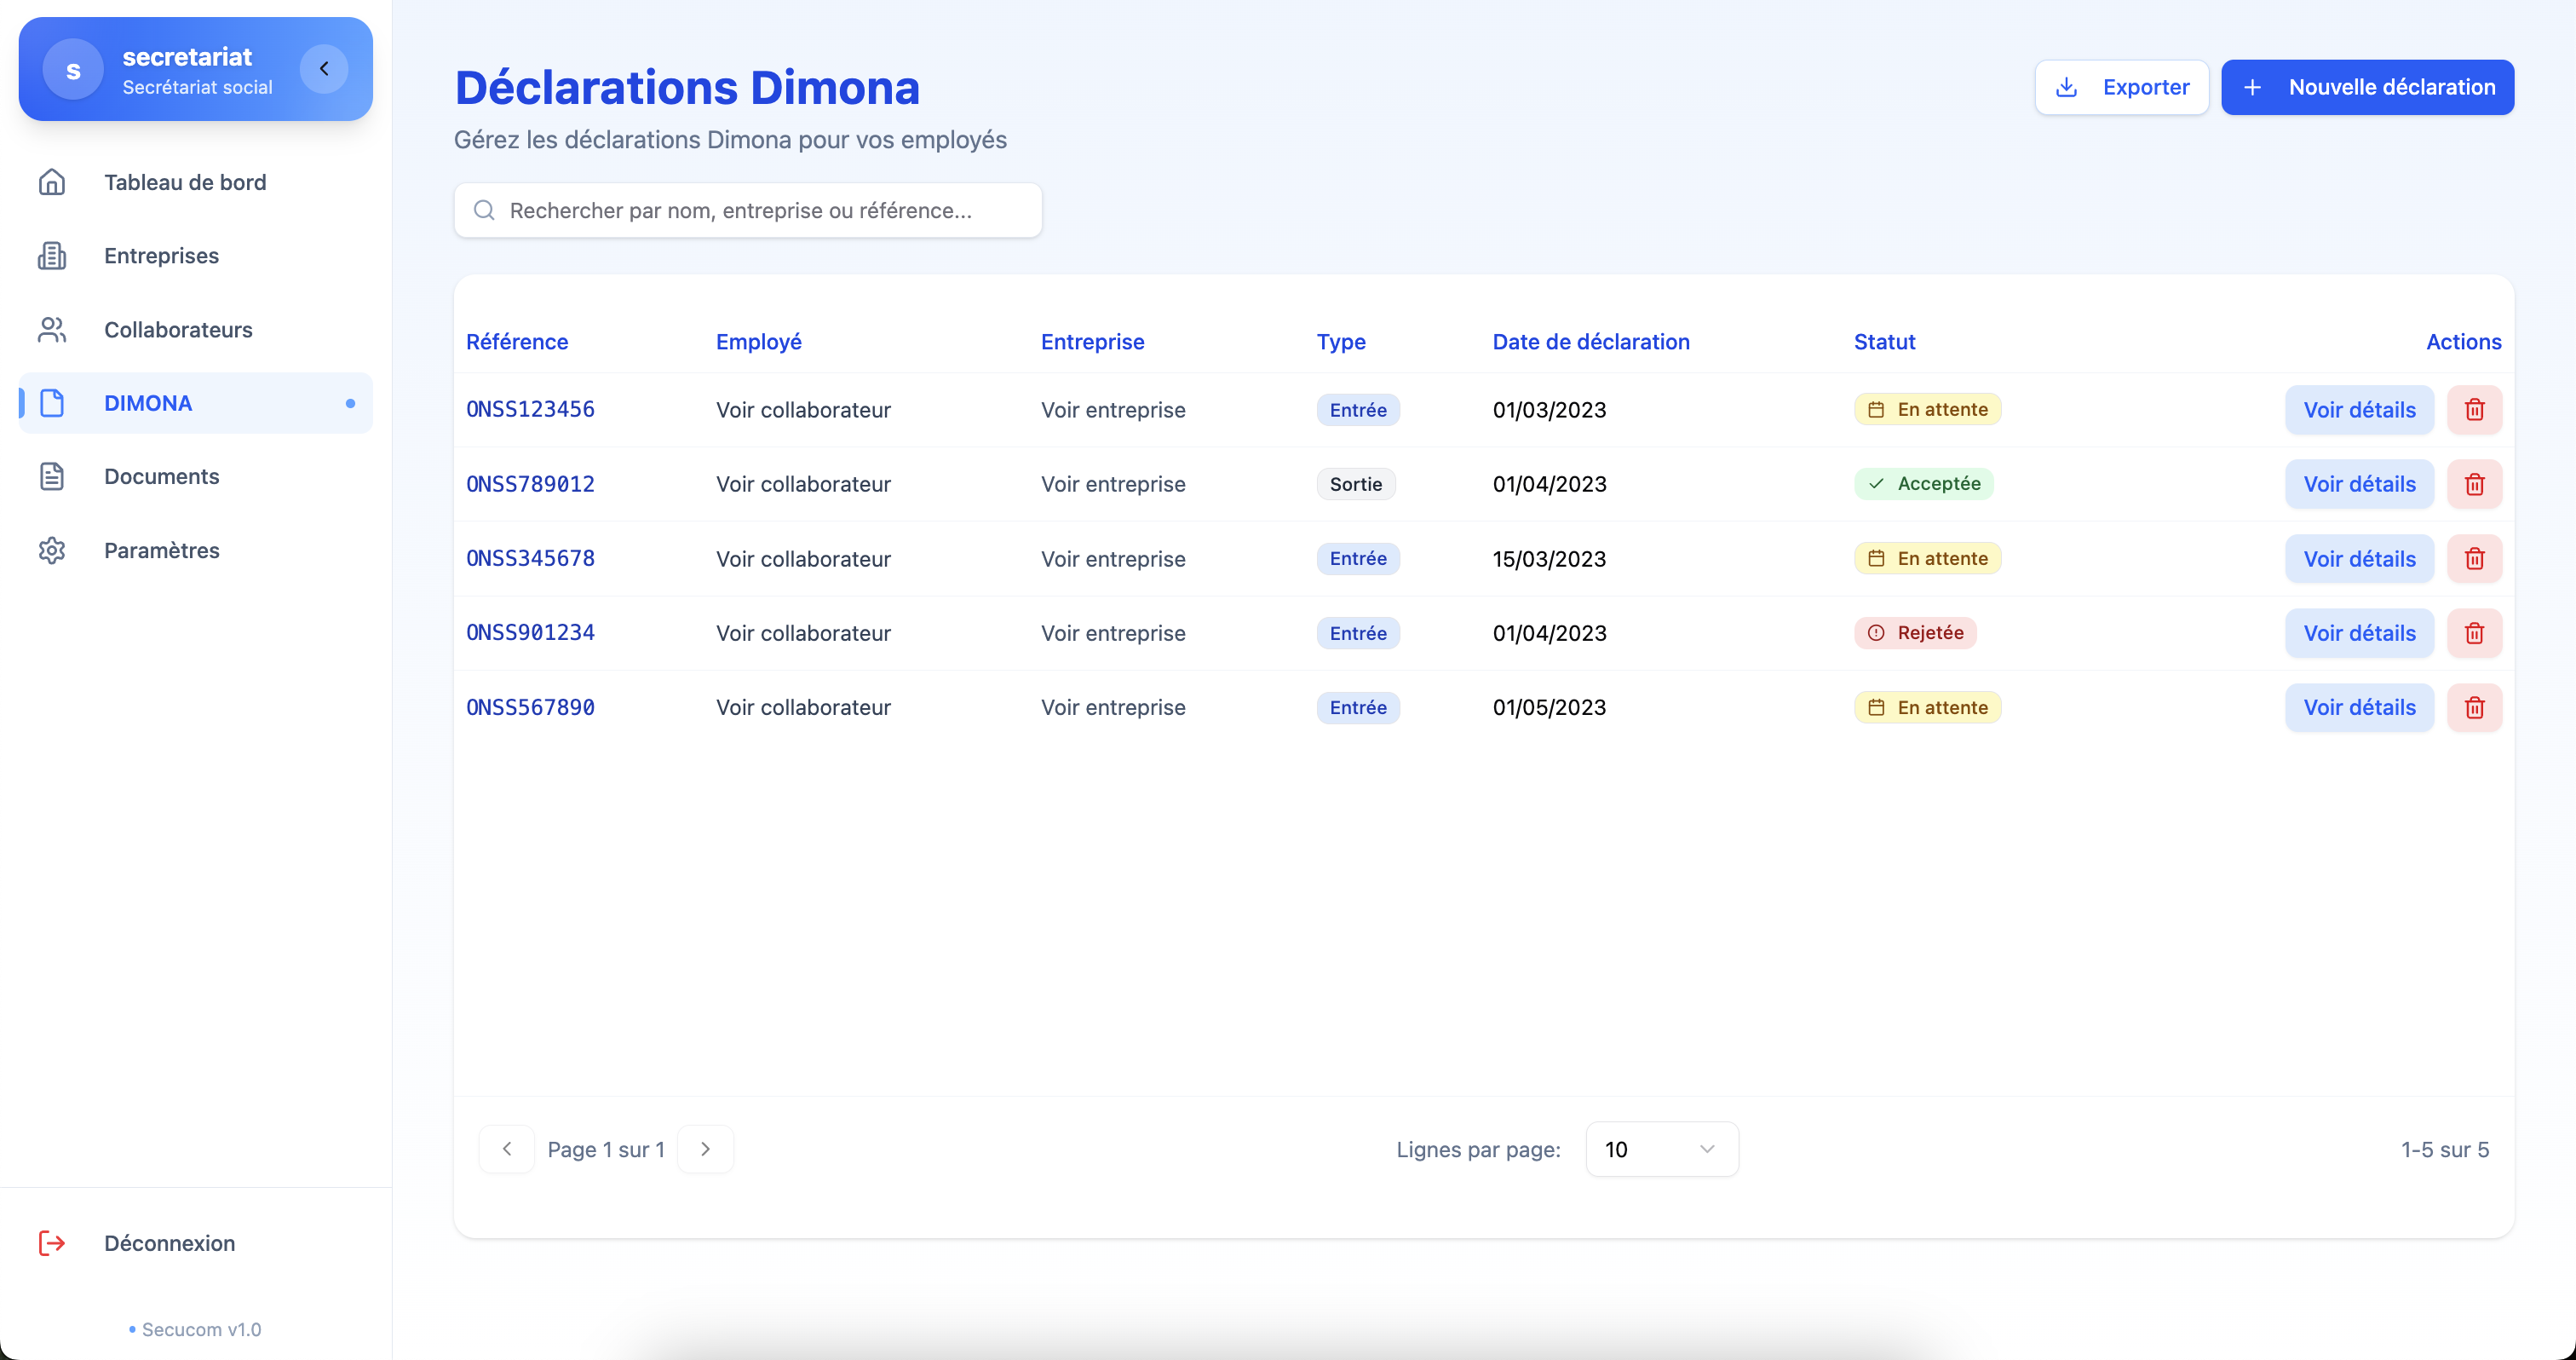
\includegraphics[width=1\textwidth]{SecuComPreviewDimona.png}
  \caption{Interface de gestion des dimonas dans SecuCom}
  \label{fig:companyInterface}
\end{figure}

\subsubsection{Modèle de données}

Le modèle de données pour les déclarations DIMONA est centré autour de l'entité \texttt{Dimona}, qui stocke les informations suivantes :

\vspace{0.5cm}

\begin{itemize}[leftmargin=*,label=\textcolor{darkgray}{$\bullet$},itemsep=0.3em]
  \item \textbf{Type de déclaration} : entrée en service, sortie de service
  \item \textbf{Dates} : dates d'entrée et de sortie
  \item \textbf{Raison de sortie} : si applicable
  \item \textbf{Statut} : 
  \item \textbf{Référence ONSS} : attribuée par l'ONSS après acceptation
  \item \textbf{Message d'erreur} : en cas de rejet
\end{itemize}

\vspace{0.5cm}

L'entité \texttt{Dimona} est liée à deux autres entités importantes :
\begin{itemize}[leftmargin=*,label=\textcolor{darkgray}{$\bullet$},itemsep=0.3em]
  \item \texttt{Collaborator} : Le travailleur concerné par la déclaration
  \item \texttt{Company} : L'entreprise employeuse
\end{itemize}

\vspace{0.5cm}

\begin{note}
Cette double association permet de retrouver facilement les déclarations par collaborateur ou par entreprise, facilitant ainsi les recherches et le reporting.
\end{note}

\subsubsection{API REST}

L'API REST pour la gestion des déclarations DIMONA est exposée par le \texttt{DimonaController}, qui offre les endpoints suivants :

\vspace{0.5cm}

\begin{tcolorbox}[
  title={\textbf{Endpoints de gestion des déclarations DIMONA}},
  colback=blue!5!white,
  colframe=primarycolor,
  fonttitle=\bfseries,
  boxrule=0.5mm,
  arc=2mm,
  left=6mm,
  right=6mm,
  top=6mm,
  bottom=6mm
]
\begin{itemize}[leftmargin=*,label=\textcolor{darkgray}{$\bullet$},itemsep=0.3em]
  \item \texttt{POST /dimona} : Création d'une nouvelle déclaration DIMONA
  \item \texttt{GET /dimona/\{id\}} : Récupération des détails d'une déclaration
  \item \texttt{GET /dimona} : Récupération de la liste des déclarations
  \item \texttt{GET /dimona/collaborator/\{collaboratorId\}} : Récupération des déclarations d'un collaborateur
  \item \texttt{GET /dimona/company/\{companyId\}} : Récupération des déclarations d'une entreprise
  \item \texttt{DELETE /dimona/\{id\}} : Suppression d'une déclaration
\end{itemize}
\end{tcolorbox}

\vspace{0.5cm}

Ces endpoints sont sécurisés et accessibles aux utilisateurs autorisés, avec des restrictions basées sur les rôles et les associations d'entreprise.

\subsubsection{Logique métier}

La logique métier pour la gestion des déclarations DIMONA est implémentée dans le \texttt{DimonaService}, qui offre les fonctionnalités suivantes :

\vspace{0.5cm}

\begin{itemize}[leftmargin=*,label=\textcolor{darkgray}{$\bullet$},itemsep=0.3em]
  \item Validation des données de déclaration (cohérence des dates, existence du collaborateur et de l'entreprise)
  \item Création des déclarations avec initialisation du statut
  \item Mise à jour du statut des déclarations après traitement par l'ONSS
  \item Récupération des déclarations avec filtrage par collaborateur ou entreprise
\end{itemize}

\vspace{0.5cm}

Le service implémente également des règles métier spécifiques, comme la vérification de la cohérence entre les dates d'entrée et de sortie, et la validation des types de déclaration selon le contexte.

\subsubsection{Processus de déclaration}

Le processus de déclaration DIMONA dans SecuCom est semi-automatisé :

\vspace{0.5cm}

\begin{tcolorbox}[
  title={\textbf{Flux de traitement d'une déclaration DIMONA}},
  colback=blue!5!white,
  colframe=primarycolor,
  fonttitle=\bfseries,
  boxrule=0.5mm,
  arc=2mm,
  left=6mm,
  right=6mm,
  top=6mm,
  bottom=6mm
]
\begin{enumerate}[itemsep=0.3em]
  \item Un utilisateur (contact d'entreprise ou employé du secrétariat) crée une demande de déclaration DIMONA dans le système.
  \item Le système valide les données et crée une entrée avec le statut "en attente".
  \item Un employé du secrétariat social traite la demande en soumettant manuellement la déclaration sur le site officiel de l'ONSS.
  \item Après traitement par l'ONSS, l'employé met à jour le statut et la référence ONSS dans le système.
  \item Le système notifie le contact d'entreprise du résultat de la déclaration.
\end{enumerate}
\end{tcolorbox}

\vspace{0.5cm}

\begin{note}
Cette approche semi-automatisée permet un contrôle humain sur les déclarations tout en bénéficiant de la validation et du suivi automatisés offerts par le système. Elle répond directement au besoin exprimé par Sodabel d'avoir un système de suivi des déclarations DIMONA.
\end{note}

\newpage
\section{Sécurité et authentification}

La sécurité est un aspect fondamental de SecuCom, étant donné la nature sensible des données traitées. L'application implémente un système robuste d'authentification et d'autorisation basé sur les tokens JWT (JSON Web Tokens).

\vspace{0.5cm}

\subsection{Authentification basée sur JWT}

L'authentification dans SecuCom est implémentée en utilisant les tokens JWT, qui offrent plusieurs avantages :
\begin{itemize}[leftmargin=*,label=\textcolor{darkgray}{$\bullet$},itemsep=0.3em]
  \item \textbf{Authentification sans état} (stateless), facilitant la scalabilité
  \item \textbf{Transmission sécurisée} des informations d'identité
  \item \textbf{Expiration automatique} des sessions
  \item \textbf{Possibilité de révocation} des tokens
\end{itemize}

\vspace{0.5cm}

\begin{tcolorbox}[
  title={\textbf{Processus d'authentification JWT}},
  colback=blue!5!white,
  colframe=primarycolor,
  fonttitle=\bfseries,
  boxrule=0.5mm,
  arc=2mm,
  left=6mm,
  right=6mm,
  top=6mm,
  bottom=6mm
]
\begin{enumerate}[itemsep=0.3em]
  \item L'utilisateur soumet ses identifiants (nom d'utilisateur/email et mot de passe) via l'endpoint \texttt{/auth/login}.
  \item Le système vérifie les identifiants et, s'ils sont valides, génère deux tokens :
    \begin{itemize}[leftmargin=*,label=\textcolor{darkgray}{$\bullet$},itemsep=0.3em]
      \item Un token d'accès (access token) de courte durée pour l'authentification
      \item Un token de rafraîchissement (refresh token) de longue durée pour obtenir de nouveaux tokens d'accès
    \end{itemize}
  \item Le token d'accès est renvoyé dans la réponse JSON, tandis que le token de rafraîchissement est stocké dans un cookie HTTP-only sécurisé.
  \item Pour les requêtes ultérieures, le client inclut le token d'accès dans l'en-tête \texttt{Authorization}.
  \item Lorsque le token d'accès expire, le client peut obtenir un nouveau token en utilisant le token de rafraîchissement via l'endpoint \texttt{/auth/refresh}.
\end{enumerate}
\end{tcolorbox}

\vspace{0.5cm}

Cette implémentation est réalisée à travers plusieurs classes :

\begin{itemize}[leftmargin=*,label=\textcolor{darkgray}{$\bullet$},itemsep=0.3em]
  \item \texttt{JwtUtils} : Génère et valide les tokens JWT
  \item \texttt{JwtAuthenticationFilter} : Intercepte les requêtes et extrait les tokens JWT
  \item \texttt{AuthController} : Expose les endpoints d'authentification
  \item \texttt{AuthService} : Implémente la logique d'authentification
  \item \texttt{UserDetailsServiceImpl} : Charge les détails utilisateur pour Spring Security
\end{itemize}

\subsection{Gestion des rôles et autorisations}

SecuCom implémente un système de contrôle d'accès basé sur les rôles (RBAC) en utilisant Spring Security. Trois rôles principaux sont définis :

\vspace{0.5cm}

\begin{table}[H]
\centering
\begin{tabular}{|l|p{10cm}|}
\hline
\textbf{Rôle} & \textbf{Description} \\
\hline
\texttt{ROLE\_ADMIN} & Administrateurs du système avec accès complet à toutes les fonctionnalités \\
\hline
\texttt{ROLE\_SECRETARIAT} & Employés du secrétariat social avec accès à toutes les entreprises clientes et leurs données \\
\hline
\texttt{ROLE\_COMPANY} & Contacts d'entreprise avec accès limité aux données de leur propre entreprise \\
\hline
\end{tabular}
\caption{Rôles utilisateurs dans SecuCom}
\end{table}

\vspace{0.5cm}

Ces rôles sont utilisés à plusieurs niveaux pour sécuriser l'application :

\begin{itemize}[leftmargin=*,label=\textcolor{darkgray}{$\bullet$},itemsep=0.3em]
  \item \textbf{Niveau URL} : Certains endpoints sont restreints à des rôles spécifiques via la configuration de Spring Security dans \texttt{SecurityConfig}.
  \item \textbf{Niveau méthode} : Des annotations comme \texttt{@PreAuthorize} sont utilisées pour sécuriser des methodes spécifiques dans les contrôleurs et services.
  \item \textbf{Niveau données} : Des filtres sont appliqués dans les services pour limiter l'accès aux données selon le rôle et l'association d'entreprise de l'utilisateur.
\end{itemize}

\vspace{0.5cm}

\begin{note}
Par exemple, un utilisateur avec le rôle \texttt{ROLE\_COMPANY} ne peut accéder qu'aux données de sa propre entreprise, tandis qu'un utilisateur avec le rôle \texttt{ROLE\_SECRETARIAT} peut accéder aux données de toutes les entreprises.
\end{note}

\subsection{Sécurisation des communications}

Toutes les communications entre le client et le serveur sont sécurisées via HTTPS/TLS, assurant la confidentialité et l'intégrité des données en transit. La configuration CORS (Cross-Origin Resource Sharing) est également mise en place pour contrôler quels domaines peuvent accéder aux ressources de l'API.

\subsection{Gestion des exceptions de sécurité}

SecuCom implémente une gestion centralisée des exceptions via \texttt{GlobalExceptionHandler}, qui intercepte les exceptions liées à la sécurité et renvoie des réponses appropriées sans exposer de détails sensibles.

\vspace{0.5cm}

\begin{tcolorbox}[
  title={\textbf{Avantages de la gestion centralisée des exceptions}},
  colback=blue!5!white,
  colframe=primarycolor,
  fonttitle=\bfseries,
  boxrule=0.5mm,
  arc=2mm,
  left=6mm,
  right=6mm,
  top=6mm,
  bottom=6mm
]
Cette approche garantit que les erreurs de sécurité sont traitées de manière cohérente et sécurisée, sans révéler d'informations qui pourraient être exploitées par des attaquants. Elle permet également de standardiser les formats de réponse d'erreur à travers toute l'application.
\end{tcolorbox}

\subsection{Protection des mots de passe}

Les mots de passe des utilisateurs sont protégés à l'aide de l'algorithme de hachage BCrypt, qui intègre automatiquement un sel (salt) unique pour chaque mot de passe, rendant les attaques par dictionnaire et par table arc-en-ciel (rainbow table) inefficaces.

\vspace{0.5cm}

\begin{note}
Lors de l'authentification, le mot de passe fourni est haché et comparé au hachage stocké, sans jamais manipuler le mot de passe en clair, conformément aux bonnes pratiques de sécurité.
\end{note}

\subsection{Audit et traçabilité}

SecuCom intègre des mécanismes d'audit pour tracer les actions importantes des utilisateurs. Les entités principales incluent des champs d'audit comme \texttt{createdAt}, \texttt{updatedAt} et \texttt{lastLogin}, qui sont automatiquement mis à jour grâce à l'annotation \texttt{@EntityListeners(AuditingEntityListener.class)}.

\vspace{0.5cm}

Cette traçabilité permet non seulement de suivre l'historique des modifications, mais aussi de détecter d'éventuelles activités suspectes et de faciliter les investigations en cas d'incident de sécurité.

\vspace{1cm}

\begin{tcolorbox}[
  title={\textbf{Sécurité transversale}},
  colback=blue!5!white,
  colframe=primarycolor,
  fonttitle=\bfseries,
  boxrule=0.5mm,
  arc=2mm,
  left=6mm,
  right=6mm,
  top=6mm,
  bottom=6mm
]
En résumé, la sécurité de SecuCom est implémentée de manière transversale à travers toutes les couches de l'application, assurant la protection des données sensibles et la conformité avec les exigences légales en matière de protection des données. Cette approche holistique de la sécurité est essentielle pour une application manipulant des données personnelles et professionnelles sensibles.
\end{tcolorbox}
